\chapter{Preliminary Material: Boson Sampling and the Schur-Weyl Duality}
\label{chp:preliminary_bs}

Parts of this chapter are joint work with Peter S. Turner, and published as ``Quantum simulation of partially distinguishable boson sampling'', \href{https://link.aps.org/doi/10.1103/PhysRevA.97.062329}{\textit{Physical Review A} \textbf{97}, 062329 (2018)}, copyright American Physics Society. Other parts of this chapter are joint work with Ra\'ul Garc\'ia-Patr\'on, Jelmer J. Renema and Peter S. Turner, and published as ``Classically simulating near-term partially-distinguishable and lossy boson sampling'', \href{https://iopscience.iop.org/article/10.1088/2058-9565/ab5555}{\textit{Quantum Science and Technology} \textbf{5}, 015001 (2020)}, copyright Institute of Physics. Preprints of these articles are freely available at {\tt \href{https://arxiv.org/abs/1803.03657}{arXiv:1803.03657}} and {\tt \href{https://arxiv.org/abs/1907.00022}{arXiv:1907.00022}}, respectively.

In the previous part of this thesis we have considered how quantum computers can offer speedups for computationally hard problems, with a particular focus on the NP-Hard Travelling Salesman Problem. But these speedups have focused on asymptotic runtimes, rather than considering how much of a speedup can be achieved in real life. This is particularly crucial when considering the issue of quantum error correction, which is a necessity for these algorithms to work in the real world.

In this part, we shift gears to focusing on an architecture-driven approach. We will focus in particular on Boson Sampling, an example of a near-term quantum architecture which is of interest due to its classical hardness rather than due to any practical applications. In Chapter \ref{chp:noisy_circuit}, we formalise a link between Boson Sampling and the representation theory of the Symmetric and Unitary groups. In doing so, we show that Boson Sampling can be modelled in the first quantisation, or particle-based picture, as sampling from a particular structure of quantum circuit, and how practical issues can be modelled as decoherence in these circuits. Then in Chapter \ref{chp:classical_sim}, we model particular kinds of imperfections in first quantisation, and show how this can lead to simpler classical simulation algorithms which we estimate will perform faster when simulating near-term devices.

The rest of this chapter is laid out as follows. We start by explaining in Section \ref{sec:error-correction} why this change in directions is necessary, by discussing practical limitations with universal quantum computation, particularly error correction. Next we introduce the topic of Quantum Advantage in Section \ref{sec:quantum-advantage}, where the focus is on non-universal models of quantum computation which seem classically hard to simulate. In Section \ref{sec:lo-bs}, we discuss linear optics and introduce the problem of Boson Sampling, an example of a Quantum Advantage proposal with strong connections to representation theory. This architecture will be the focus of this part. Experimental achievements are given in Section \ref{sec:experimental-achievements}, as well as limitations with larger experiments and how these lead to classical simulations in Sections \ref{sec:lo-imperfections} and \ref{sec:classical-simulations}. We will conclude this chapter summarising some ideas in representation theory, in particular the Quantum Schur Transform, in Section \ref{sec:sw-duality}. Although the switch to representation theory at the end of this chapter might seem at odds with the rest of this chapter, we will show in Chapters \ref{chp:noisy_circuit} and \ref{chp:classical_sim} how these two subjects relate to one another.

\section{Estimated speedups in practice and the limitations of quantum error correction}
\label{sec:error-correction}

At the same time as pursuing theoretical speedups through algorithms such as those described in Chapters \ref{chp:prelim-q-c} and \ref{chp:tsp}, it is worth questioning the extent to which these algorithms can provide speedups in real-world scenarios. Ideally we want a situation where a quantum computer would be able to solve a problem with relevant applications significantly faster than a classical computer.

The question of whether or not NP-Hard problems can fit this scenario was considered by Campbell, Khurana and Montanaro \cite{campbell2019}, who looked at estimating the resources required for Grover search and Montanaro's backtracking algorithm when applied to the problems of boolean satisfiability and graph colouring. Campbell, Khurana and Montanaro provided a gate decomposition for these two algorithms when running for random problem instances under different assumptions about the quantum hardware, from realistic scenarios to more optimistic ones. These estimated runtimes were then compared with the best classical solvers for boolean satisfiability and graph colouring. From this, Campbell, Khurana and Montanaro came up with the largest problem sizes that these models could solve in a day, and showed that a speedup could potentially be achieved: For SAT, the estimated improvement in the optimistic scenario was as much as $100,000$ faster, and a $10,000$ times speedup was estimated for graph colouring \cite{campbell2019}.

However, there is also a cost that comes with running these algorithms for the largest problem sizes: how much error correction is required to reliably solve the problem. This was estimated using a gate decomposition of Clifford gates as well as either the single qubit $T$ gate or the three-qubit Toffoli gate as non-Clifford operations which can provide universal quantum computation. The idea is that one can use the surface code to implement any Clifford gates in a fault-tolerant fashion, and then the non-Clifford gates can be implemented by preparing a particular quantum state, called a magic state, and then using that state in the rest of the Clifford operations. This means that the only significant overhead is in the preparation of these magic states, which is done via a purification technique where less ideal magic states are used to construct more ideal states. The qubits required to produce these states are known as the factory qubits.

Unfortunately the result of Campbell, Khurana and Montanaro shows that the number of magic states required in these instances is significant \cite{campbell2019}. For the $10^5$ speedup mentioned earlier, a total of $10^{19}$ Toffoli gates is required, corresponding to $10^{12}$ factory qubits. Similarly for graph colouring, the $10^4$ speedup requires on the order of $10^{20}$ $T$ or Toffoli gates, and $10^{12}$ factory qubits. What is even more concerning is that implementing so many Toffoli or $T$ gates also requires a significant amount of classical processing: Campbell, Khurana and Montanaro showed that the classical processing required to implement $10^{20}$ Toffoli gates was on the order of $10^8$ processor days even for specialised electronics such as application-specific integrated circuits. For a standard CPU, this overhead could be as large as $10^{16}$ processor days. Such a large overhead means that any quantum advantage from these techniques would immediately be lost.

A potential workaround for this is adapting quantum algorithms to near-term architectures. There are a small number of results in this area, particularly when the number of logical qubits required is small. Dunjko, Ge and Cirac \cite{dunjko2018} showed that a polynomial (at most quadratic) speedup for Satisfiability can be shown for a quantum computer of arbitrary size. This was achieved by first using classical backtracking to reduce the Boolean formula to problem instances small enough that they can be run on the quantum computer, and then applying Grover search to obtain a quadratic speedup for these smaller instances. Ge and Dunjko \cite{ge2019} later developed a general framework based on this idea, and showed how it can be applied to find Hamiltonian cycles in bounded-degree graphs, achieving a polynomial speedup over Eppstein's algorithm \cite{eppstein2007}\footnote{It is worth noting that this speedup is not at most a quadratic one over Eppstein's algorithm. This is because the approach of Ge and Dunjko uses Grover search instead of the quantum backtracking algorithms.}. However these algorithms still require logical qubits, and therefore might use a large number of physical qubits to operate in practice.

\section{The search for a quantum advantage}
\label{sec:quantum-advantage}

So if fault tolerant quantum computing is not currently an option, this begs the question of what is achievable without it, and in particular what can be performed exponentially faster than classical computers in spite of having little or no error correction.

This is a concept that has gone through a few different names, most notably ``quantum computational supremacy.'' In this chapter and throughout the rest of this thesis, we shall use the term ``quantum advantage'' to refer to this area, and refer the reader to \cite{wiesner2017, palaciosberraquero2019} for further discussion of the issues surrounding the use of ``supremacy.'' Here, the emphasis is on finding a model of quantum computation that is hard to classically simulate. Such a quantum computer need not be universal, or even have practical applications. However, it should be provably hard to simulate classically, under reasonable assumptions, and with little to no error correction required.

For simplicity, we shall not detail the formal proofs of different quantum advantage problems, and instead note a general structure of the proofs of hardness. These problems are typically described as sampling problems, where the aim is to produce an output from (approximately) the same probability distribution as the quantum computer. For these proofs to work, we require that approximating one of these probabilities is $\sharpp$-Hard. If this is true, then a result of Stockmeyer \cite{stockmeyer1983} shows that classically being able to sample from this exact distribution leads to a algorithm that can approximate these probabilities up to a multiplicative error. This would imply a model of computer which can approximately solve $\sharpp$-Hard problems, which in turn would lead to the collapse of the Polynomial Hierarchy to the third level by Toda's Theorem \cite{toda1991}. This consequence is similar to, though not as strong as, $\p=\np$, and is considered equally unlikely.

This proves that if sampling from the exact distribution can be done classically, then the Polynomial Hierarchy collapses to the third level. However, we often want to go further than this claim, and show that to even sample from a distribution which is approximately equal to the target distribution is hard.

Before explaining how to prove the hardness of approximate sampling, it is worth discussing what it means to sample from an approximate distribution in the first place. For this, we use the total variation distance, which is defined between two probability distributions $P$ and $Q$ over a finite set of outcomes $\Omega$ as half the $L_1$ distance:

\begin{equation}
\Delta(P, Q) \colon= \frac{1}{2}\sum_{\omega \in \Omega}|P(\omega) - Q(\omega)|.
\end{equation}

Another distance which is also used particularly for quantum states is the trace distance, which is defined between two states $\rho$ and $\sigma$ as

\begin{equation}
\delta_{\trace}(\rho, \sigma) \colon= \frac{1}{2}\trace\left[\sqrt{(\rho-\sigma)^\dagger(\rho-\sigma)}\right].
\end{equation}

The trace distance can also be defined as the maximum total variation distance between any two states when a measurement is applied is applied:

\begin{equation}
\delta_{\trace}(\rho, \sigma) \colon= \max_E\Delta(E(\rho), E(\sigma)),
\end{equation}

\noindent where $E$ is taken over all positive operator valued measures. As a result, it is often beneficial to use the trace distance as an upper bound for the total variation distance. We can also note that this distance is convex:

\begin{equation}
\delta_{\trace}(\rho, \sigma + \tau) \leq \delta_{\trace}(\rho, \sigma) + \delta_{\trace}(\rho, \tau).
\end{equation}

As well as understanding how we measure the distance between two distributions, it is worth discussing the size of the error. Let $p \in [0,1]$ be our target probability for some outcome, and $\tilde{p} \in [0,1]$ be its approximation. For some $\epsilon > 0$, we say that $p$ and $\tilde{p}$ are approximately equal up to additive error $\epsilon$ if $|p-\tilde{p}|\leq \epsilon$, and approximately equal up to multiplicative error $\epsilon$ if $|p-\tilde{p}|\leq p\epsilon$. It is easy to see that multiplicative error immediately implies additive error as well, but additive error does not necessarily imply multiplicative error.

We are now ready to define approximate sampling. We say that a target distribution $P$ can be approximately sampled from efficiently if there is a probability distribution $\tilde{P}$ which can be sampled from in polynomial time and is approximately equal to $P$ in total variation distance up to additive error $\epsilon$ for some $\epsilon > 0$:

\begin{equation}
\Delta(P, \tilde{P}) \leq \epsilon.
\end{equation}

To prove that even approximately sampling is hard, we require two further assumptions, in order to reduce sampling from the target distribution to sampling from the approximate distribution. The first is the distribution must anticoncentrate; this means that the distribution is largely spread out rather than having peaks\footnote{Note however that the distribution cannot be too far spread out, otherwise it becomes close to the uniform distribution which can be sampled classically.}. The second is that approximating the probability of a random outcome up to multiplicative error must be hard, not just the worst-case outcome. Using these two assumptions, we can reduce from an exact sampling problem to an approximate one, and then use the argument above to show that even approximately sampling must be hard for the Polynomial Hierarchy to not collapse. Intuitively, these assumptions ensure that a polynomial-time classical simulator cannot simply sample from the peaks of the distribution (by anticoncentration), nor can it just sample from the outcomes whose probabilities are easy to approximate (average-case hardness).

As we shall see in Sections \ref{ssec:qa-examples} and \ref{ssec:cc-bs}, each of the problems have more or less the same argument as that stated above, though what is proven and what remains conjecture tends to vary. It has been proven for some sampling problems that their distributions do anticoncentrate, and it has been proven for some problems that exactly computing the probability of a random outcome is $\sharpp$-hard. What has not currently been proven for any quantum advantage problem is that it is $\sharpp$-hard to approximate the probability of a random outcome, though we have some idea of what techniques will not lead to a successful proof. Aaronson and Chen \cite{aaronson2016chen} proved two details, regarding the use of oracles\footnote{An oracle in complexity theory is a process that an algorithm can query. The overall runtime is the overhead of the algorithm, plus the number of oracle queries multiplied by the oracle's runtime for each query.} in such a proof. The first is that a proof cannot be relative to arbitrary oracles, as there exists an oracle relative to which the complexity classes of classical probabilistic sampling and quantum sampling are equivalent, yet the Polynomial Hierarchy does not collapse. The second is that if the proof is restricted to using an oracle in $P$ with a polynomial advice string that only depends on the size of the input, then in order for the Polynomial Hierarchy to collapse we need to assume that either classical and quantum sampling complexity are not equivalent, in which case an oracle is not necessary, or $\np \nsubseteq \bpp$, where $\bpp$ is the class of what can be solved in polynomial time probabilistically with bounded error. This second assumption is a closely related to a standard assumption in cryptography: That there are functions which are easy to compute but hard to invert, also known as one-way functions.

Note that while these proofs rule out polynomial classical simulations of Quantum Advantage problems, they do not state the point at what size these problems become intractable. This requires a more fine-grained approach to the computational complexity conjectures. Dalzell et al.~\cite{dalzell2017, dalzell2018} gave such an approach, devising conjectures similar to the Strong Exponential Time Hypothesis mentioned in Chapter \ref{chp:prelim-q-c}, and providing fine-grained lower bounds by showing that a classical simulator running in a certain time with polynomial multiplicative error could violate these conjectures. From this, Dalzell et al.\ estimate the largest such instances that a modern supercomputer could classically simulate in a century, based on number of floating point operations required. The requirement of simulating up to multiplicative error is strong, but some very recent work by Morimae and Tamaki has given similar results for certain problems with additive error \cite{morimae2019}.

Another interesting question, though one that will not be explored in great detail in this thesis, is the question of verifying a quantum advantage. That is, given a collection of samples from some distribution, how do we check that this is the (known) target distribution we want, instead of some other (classical) distribution. This is a challenge, primarily for the same reasons that it is hard to simulate these problems in the first place: a combination of having many probabilities close to uniform and the fact that even estimating one probability is exponentially hard. Indeed, Hangleiter et al.~\cite{hangleiter2019} showed that for any sufficiently flat distribution, verifying the distribution purely from samples and a description of the target distribution must require exponentially many samples.

\subsection{Example problems}
\label{ssec:qa-examples}

We will now describe some example problems related to Quantum Advantage, and explain what is currently known about them.

\begin{problem}[Instantaneous Quantum Polynomial Time (IQP) Circuit Sampling] Let $C$ be an $n$-qubit polynomial time quantum circuit consisting only of nearest-neighbour controlled phase gates in a 2D lattice. Sample from the distribution corresponding to measuring the state

\begin{equation}
H^{\otimes n}CH^{\otimes n}|0\rangle^{\otimes n}
\end{equation}
\noindent in the computational basis.
\end{problem}

IQP circuits were originally proposed by Shepherd and Bremner \cite{shepherd2009thesis, shepherd2009}, where some applications were proven and the circuits were conjectured to be classically hard. This was followed up in 2011, when Bremner, Jozsa and Shepherd proved that efficient classical simulation led to the collapse of the Polynomial Hierarchy, assuming anticoncentration and average-case hardness conjectures \cite{bremner2011}. The anticoncentration conjecture was proven to hold by Bremner, Montanaro and Shepherd \cite{bremner2016}.

It is worth noting that these IQP circuits required controlled phase gates between arbitrary qubits. The more restricted form defined above was given by Bremner, Montanaro and Shepherd in 2017 \cite{bremner2017}, showing that a circuit of $O(\sqrt{n}\log n)$ depth implemented on a 2D lattice anticoncentrates and fits the hardness arguments above. They also considered noise in such a circuit, and gave two further results: One, that an average IQP circuit with $\epsilon$ depolarising noise applied to each qubit can be simulated with accuracy $\delta$ in time polynomial in $n$; and two, that a simple form of error correcting code can manage to retain classical hardness even when faced with depolarising noise.

\begin{problem}[Random Circuit Sampling] Let $C$ be a random circuit of depth $O(n)$ which consists of random 1- and 2-qubit operations from a universal gate set applied to nearest neighbours on a 2D lattice. Sample from the distribution corresponding to measuring the state $C|0\rangle^{\otimes n}$ in the computational basis.
\end{problem}

Random Circuit Sampling is a model first proposed by Boixo et al.~\cite{boixo2018}, motivated by the superconducting quantum computing architecture developed by Google. In their result, Boixo et al.\ argue that it is computationally hard to classical sample from this distribution under anticoncentration and average-case hardness assumptions, used numerical simulations to give reason to believe that $O(\sqrt{n})$-depth circuits are sufficient for the distribution to anticoncentrate, and proposed a verification metric called the cross entropy difference. Since their publication, the anticoncentration conjecture was proven to hold by Hangleiter et al.~\cite{hangleiter2018}, and exactly computing the probability of an outcome was proven to be $\sharpp$-hard on average by Bouland et al.~\cite{bouland2018}. Most recently, Random Circuit Sampling has been the centre of interest due to a publication by Arute et al.\ who implemented the problem on Google's 54 qubit quantum processor, claiming that this is now of a size that cannot be simulated by classical computers \cite{arute2019}. This was verified by estimating a property known as the cross-entropy fidelity, a metric proposed by Boixo et al.~\cite{boixo2018} and later proven hard to classically spoof by Aaronson and Gunn \cite{aaronson2019}. However, it is worth noting that there is some rebuttal from Pednault et al.\ at IBM \cite{pednault2019}, who claim that given sole use of the Summit supercomputer at Oak Ridge National Laboratory classical simulations could be achieved in two and a half days, and argue that this isn't sufficient for the claim of quantum advantage. Likewise, a report by Morimae, Takeuchi and Tani \cite{morimae2019google} suggests that the fidelity is sufficiently low that simply sampling from the uniform distribution would be sufficiently precise in this case.

\section{Linear optics and Boson Sampling}
\label{sec:lo-bs}

So far in this chapter we have motivated the need for pratical sampling experiments which can offer a quantum advantage. We now move to explaining the problem of interest for this part of the thesis: Boson Sampling. We will start by explaining the theory of linear optics and some simple example interferometers, before introducing Boson Sampling and discussing its classical complexity, as well as briefly summarising some variants which use non-linear photonic inputs.

\subsection{Single photons and linear optical components}

Boson Sampling experiments can be developed from the use of single photons, simple linear optical components and single photon detectors. We shall now summarise how such photons and components can be described in both second and first quantisation. For a more thorough understanding of these concepts we direct the interested reader to \cite{fox2006, gerry2012}.

\subsubsection{Second quantisation}

We shall start with second quantisation, as the more common and natural way of describing bosonic systems. The bosonic Fock space follows a direct sum of symmetric tensors:

\begin{equation}
F(H) = \oplus_{n=0}^\infty\textrm{Sym}(H^{\otimes n}),
\end{equation}

\noindent where $H$ is a Hilbert space, and $\textrm{Sym}$ denotes the symmetric subspace.

An $m$-mode bosonic Fock state is written as an $m$-dimensional complex vector $\ket{S_1,S_2,\dots,S_m}$, where $S_i$ is the number of photons occupying mode $i$. The number of photons in mode $i$ can be decremented or incremented by annihilation and creation operations $a_i$ and $a_i^\dagger$, respectively:

\begin{equation}
a_i\ket{S_1,\dots,S_i,\dots,S_m} = \sqrt{S_i}\ket{S_1,\dots,S_i-1,\dots,S_m},
\end{equation}

\begin{equation}
a_i\ket{S_1,\dots,S_i,\dots,S_m} = \sqrt{S_i+1}\ket{S_1,\dots,S_i+1,\dots,S_m}.
\end{equation}

We also have the commutation relations $[a_i^\dagger, a_j^\dagger] = [a_i,a_j] = 0$ and $[a_i^\dagger, a_j] = \delta_{ij}$.

A particular Fock occupation can therefore be described by creation operators acting on the vacuum state:

\begin{equation}
\ket{S_1,\dots,S_m} = \prod_{i=0}^m\frac{(a_i^\dagger)^{S_i}}{\sqrt{S_i!}}\ket{0^m},
\end{equation}

\noindent where we have used the shorthand notation

\begin{equation}
\ket{i^j} = \ket{\overbrace{i,i,i,\dots,i}^{j \textrm{ copies}}}.
\end{equation}

We shall use these creation and annihilation operators to describe how we apply optical components to act on the initial state.

There are two basic linear optical components we require to implement Boson Sampling. The first is a phase shifter, which induces a phase on a spatial mode. A phase shifter on mode $j$ induces:

\begin{equation}
a_j^\dagger \rightarrow e^{i\theta}a_j^\dagger.
\end{equation}

Physically, a phase shifter can be implemented as a change of refractive index, which can speed up or slow down the transmission of light.

The second component is a beam splitter. This component acts as a partial mirror between two spatial modes, transmitting some light and reflecting other light. A beam splitter on spatial modes $j$ and $k$ with reflectivity $r, r'$ and transmittance $t, t'$ acts as the following:

\begin{equation}
a_j^\dagger \rightarrow ta_j^\dagger + r'a_k^\dagger,
\end{equation}

\begin{equation}
a_k^\dagger \rightarrow ra_j^\dagger + t'a_k^\dagger,
\end{equation}

\noindent where we have the constraints that $|r|=|r'|, |t|=|t'|, |r|^2+|t|^2=1$ and $r^*t' + r't^* = r^*t+r't'^*=0$. Of particular note is the 50-50 beam splitter, where exactly half the light is reflected and the other half is transmitted. In this case, $r=r'=1/\sqrt{2}$ and $t=t'=i/\sqrt{2}$. Note the $\pi/2$ phase difference between reflection and transmission, which is important for the interferometers we shall be discussing in Section \ref{ssec:example-interferometers}.

Finally, we need to measure the number of photons in each spatial mode. To do this, we can use the photon number measurement $n_i = a_i^\dagger a_i$. It can be seen that this operator is Hermitian and its eigenvectors are the Fock basis for mode $i$, with eigenvalues depending on the number of photons occupying mode $i$. For example, if there are $j$ photons in mode $i$ we see that

\begin{align}
n_i\ket{j} &= a_i^\dagger a_i\ket{j}\\
&= \sqrt{j}a_i^\dagger\ket{j-1}\\
&= \sqrt{j}\sqrt{j-1+1}\ket{j-1+1}\\
&= j\ket{j}.
\end{align}

Any linear optical interferometer can be composed from the above components, as we shall see in Section \ref{ssec:universal-lo} \cite{hurwitz1897, reck1994, clements2016}.

\subsubsection{First quantisation}

Equivalently, we can describe these effects in the first quantisation, or particle-based, picture. In this picture, our input is a state in the symmetric subspace of $\mathbb{C}^{m\times n}$. This means that each of our $n$ particles is represented as am $m$-dimensional qudit, and the overall state has to be symmetric as no single particle can be uniquely identified. For example, the Fock state $\ket{2,0}$ corresponds to the first quantised state $\ket{11}$, whereas the Fock state $\ket{1,1}$ corresponds to $(\ket{12} + \ket{21})/\sqrt{2}$. In general, the Fock state $\ket{S_1,\dots,S_m}$ corresponds to

\begin{equation}
\frac{1}{\sqrt{n!\prod_{i=1}^mS_i!}}\left(\sum_{\sigma\in\symm_n}\sigma\bigotimes_{j=1}^m\ket{j}^{\otimes S_j}\right),
\end{equation}

\noindent where $\symm_n$ means the Symmetric group, or number of ways of permuting $n$ objects. Linear optical components can now be applied to each particle individually as an $m \times m$ unitary matrix. For example, the action of a $\theta$-phase shifter applied to one mode in a two-mode interferometer can be written as

\begin{equation}
\begin{pmatrix}
e^{i\theta} & 0\\
0 & 1
\end{pmatrix}.
\end{equation}

The action of a beam splitter with reflectivity $r, r'$ and transmittance $t, t'$ can be written as

\begin{equation}
\begin{pmatrix}
t & r'\\
r & t'
\end{pmatrix},
\end{equation}

\noindent with the same restraints as in first quantisation. Of particular note, the 50-50 beam splitter has unitary matrix

\begin{equation}
\begin{pmatrix}
\frac{1}{\sqrt{2}} & \frac{i}{\sqrt{2}}\\
\frac{i}{\sqrt{2}} & \frac{1}{\sqrt{2}}
\end{pmatrix}.
\end{equation}

Finally, a photon number counting measurement simply consists of measuring each qudit in the computational basis and counting the number of qudits in each state $j \in \{1,\dots,m\}$.

\subsection{Example linear optical interferometers}
\label{ssec:example-interferometers}

We shall now discuss some example interferometers, and their resulting effects, using the notation described above. This will eventually lead us to talk about Boson Sampling in Section \ref{ssec:bosonic-sampling}.

\subsubsection{One-photon-two-modes: The Mach-Zehnder Interferometer}

\begin{figure}
\subfloat[\label{fig:mzi-diagram}]{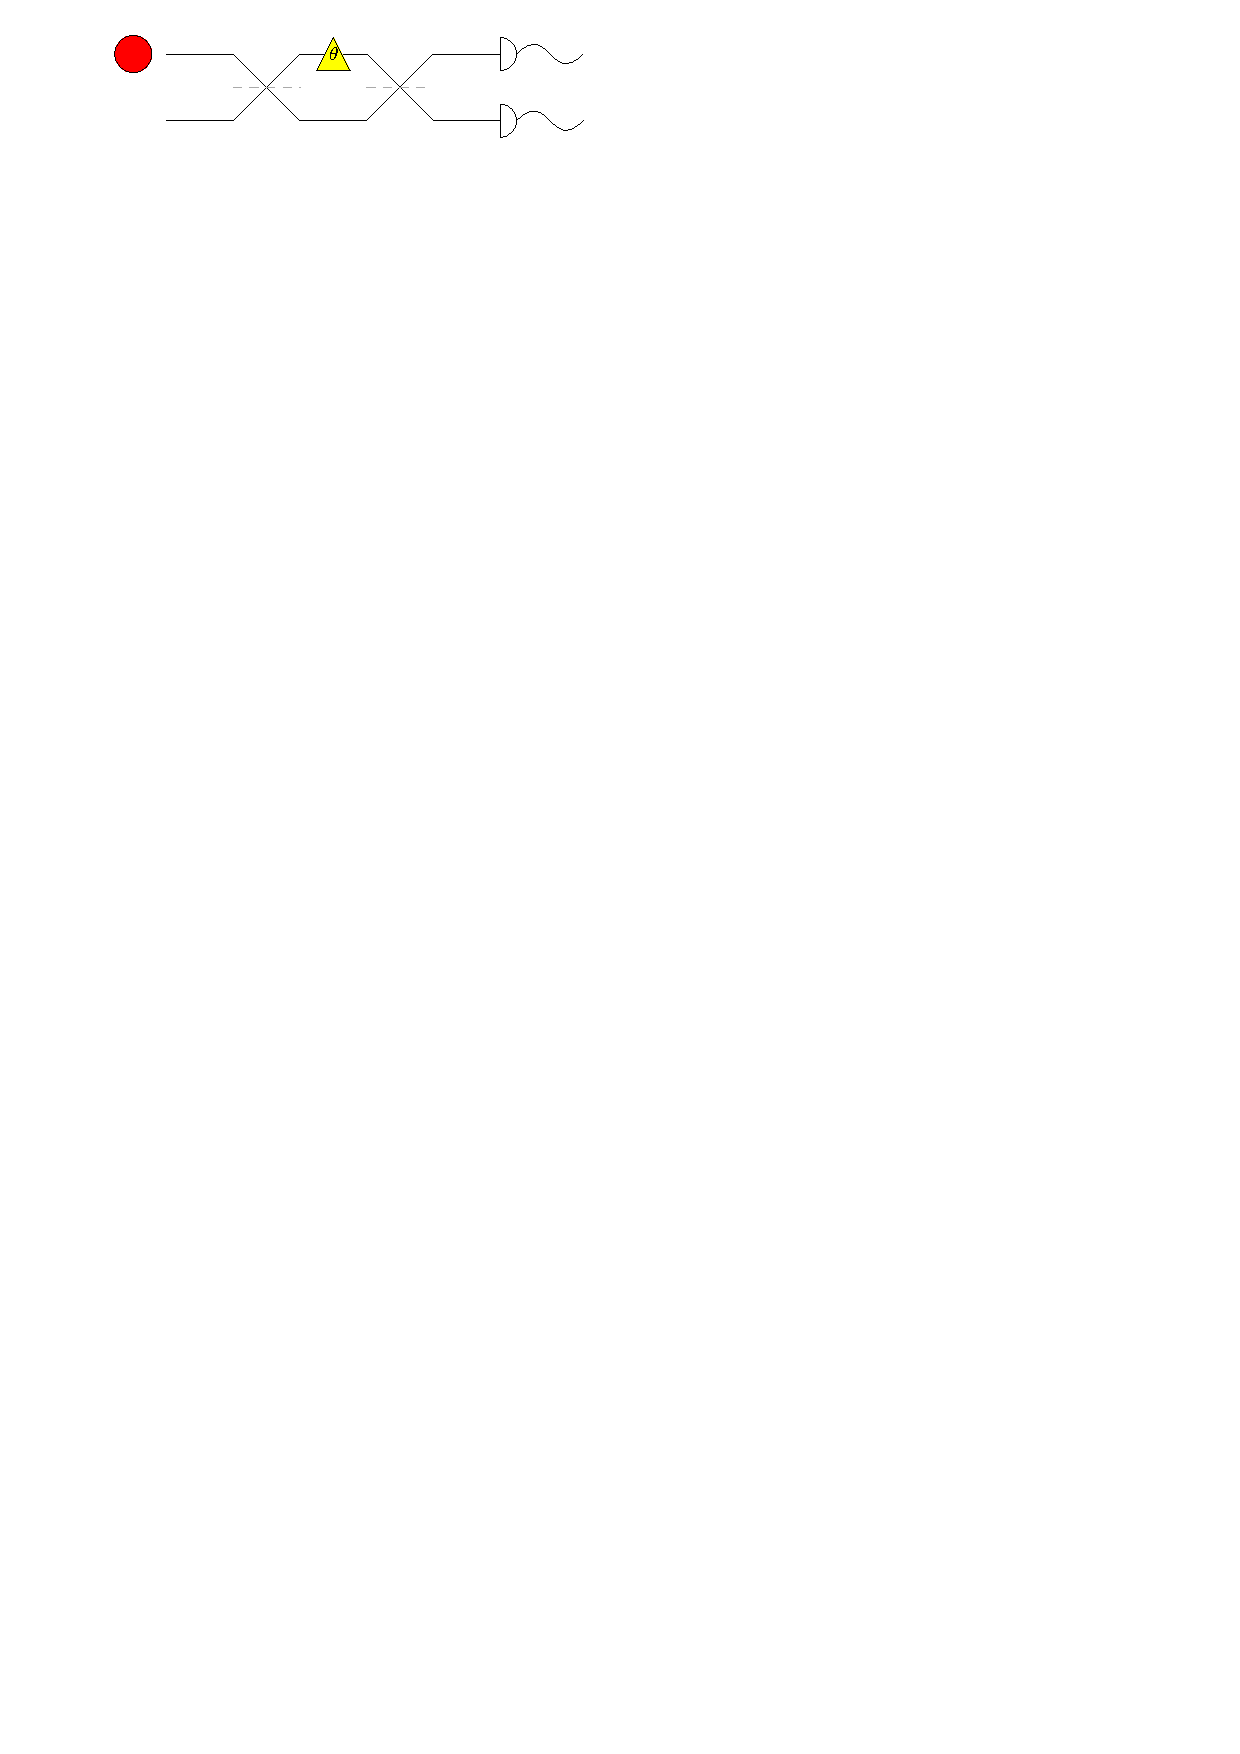
\includegraphics[width=0.45\linewidth]{preliminary_bs/mzi}}
\hfill
\subfloat[\label{fig:mzi-plot}]{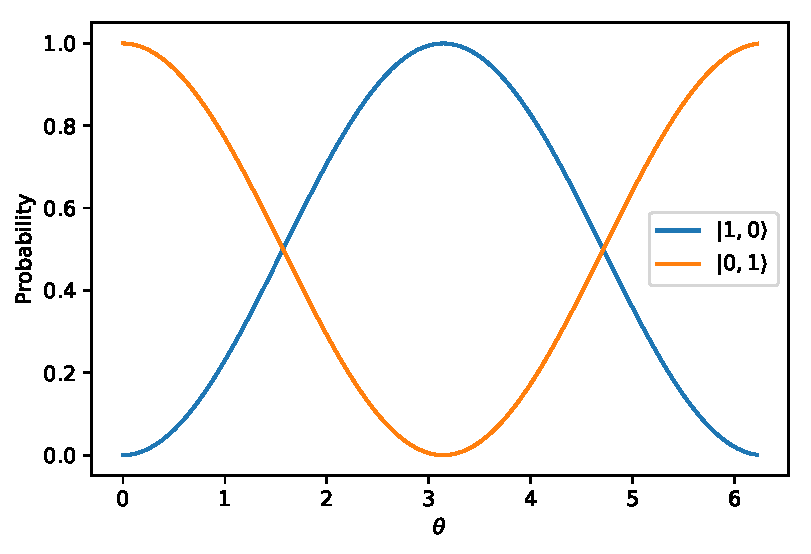
\includegraphics[width=0.45\linewidth]{preliminary_bs/mzi_plot}}
\caption[Experimental setup of the Mach-Zehnder Interferometer and probability of outcomes over phase $\theta$]{\label{fig:mzi}The Mach-Zehnder Interferometer, a demonstration of single-photon interference. \ref{fig:mzi-diagram}: An experimental diagram, consisting of a single photon (red circle) in one of two spatial modes (solid black lines), a phase shifter (yellow triangle containing $\theta$) surrounded by two 50-50 beam splitters (grey dashed lines) and single photon detectors (white semi-circles). \ref{fig:mzi-plot}: The Probability of measuring $\ket{0,1}$ (orange) and $\ket{1,0}$ (blue) from a Mach-Zehnder Interferometer over $\theta$.}
\end{figure}

A Mach-Zehnder Interferometer (MZI) is a demonstration of how a single photon can interfere with itself \cite{zehnder1891,mach1892}. This experiment uses a single photon in one of two modes, and consists of a 50-50 beam splitter across both modes, followed by a phase shifter on a single mode, and finally a second 50-50 beam splitter. A diagram of this experiment can be seen in Figure \ref{fig:mzi-plot}.

In second quantisation, we can describe the MZI as follows, labelling our spatial modes 1 and 2. We start with a single photon in mode 1 $\ket{1,0} = a_1^\dagger\ket{0,0}$. After our first beam splitter we have the state $(a_1^\dagger + ia_2^\dagger)\ket{0,0}/\sqrt{2}.$

We next apply a phase shifter to spatial mode 1, giving $(e^{i\theta}a_1^\dagger + ia_2^\dagger)\ket{0,0}/\sqrt{2}$. Finally, we apply our second beam splitter and find that

\begin{align}
\frac{1}{\sqrt{2}}(e^{i\theta}a_1^\dagger + ia_2^\dagger)\ket{0,0} &\rightarrow \frac{1}{2}(e^{i\theta}(a_1^\dagger+ia_2^\dagger) + i(ia_1^\dagger + a_2^\dagger))\ket{0,0}\\
&= \frac{1}{2}((e^{i\theta}-1)a_1^\dagger+i(e^{i\theta}+1)a_2^\dagger)\ket{0,0}.
\end{align}

Adjusting our phase $\theta$ determines what output we measure: For $\theta=0$, the photon will be in mode 2; for $\theta=\pi/2$, the photon will be in mode 1, and for other values of $\theta$ the photon will be measured randomly in one of the two modes. How the probabilities change over $\theta$ is given in Figure \ref{fig:mzi-plot}.

In first quantisation, we see the same outcome. Our input is $\ket{1}$, and  applying the first beam splitter leads to the state $(\ket{1}+i\ket{2})/\sqrt{2}$. The phase shifter on mode 1 results in the state $(e^{i\theta}\ket{1}+i\ket{2})/\sqrt{2}$, and the second beam splitter leaves us with the state

\begin{align}
\ket{\psi} &= \frac{1}{2}\left(e^{i\theta}\left(\ket{1} + i\ket{2}\right) + i\left(i\ket{1} + \ket{2}\right)\right)\\
&= \frac{1}{2}\left(\left(e^{i\theta}-1\right)\ket{1} + i\left(e^{i\theta}+1\right)\ket{2}\right).
\end{align}

Again, we see that adjusting $\theta$ will determine which spatial mode we detect a photon in.

\subsubsection{Two-photons-two-modes: The Hong-Ou-Mandel Dip}

\begin{figure}
\begin{center}
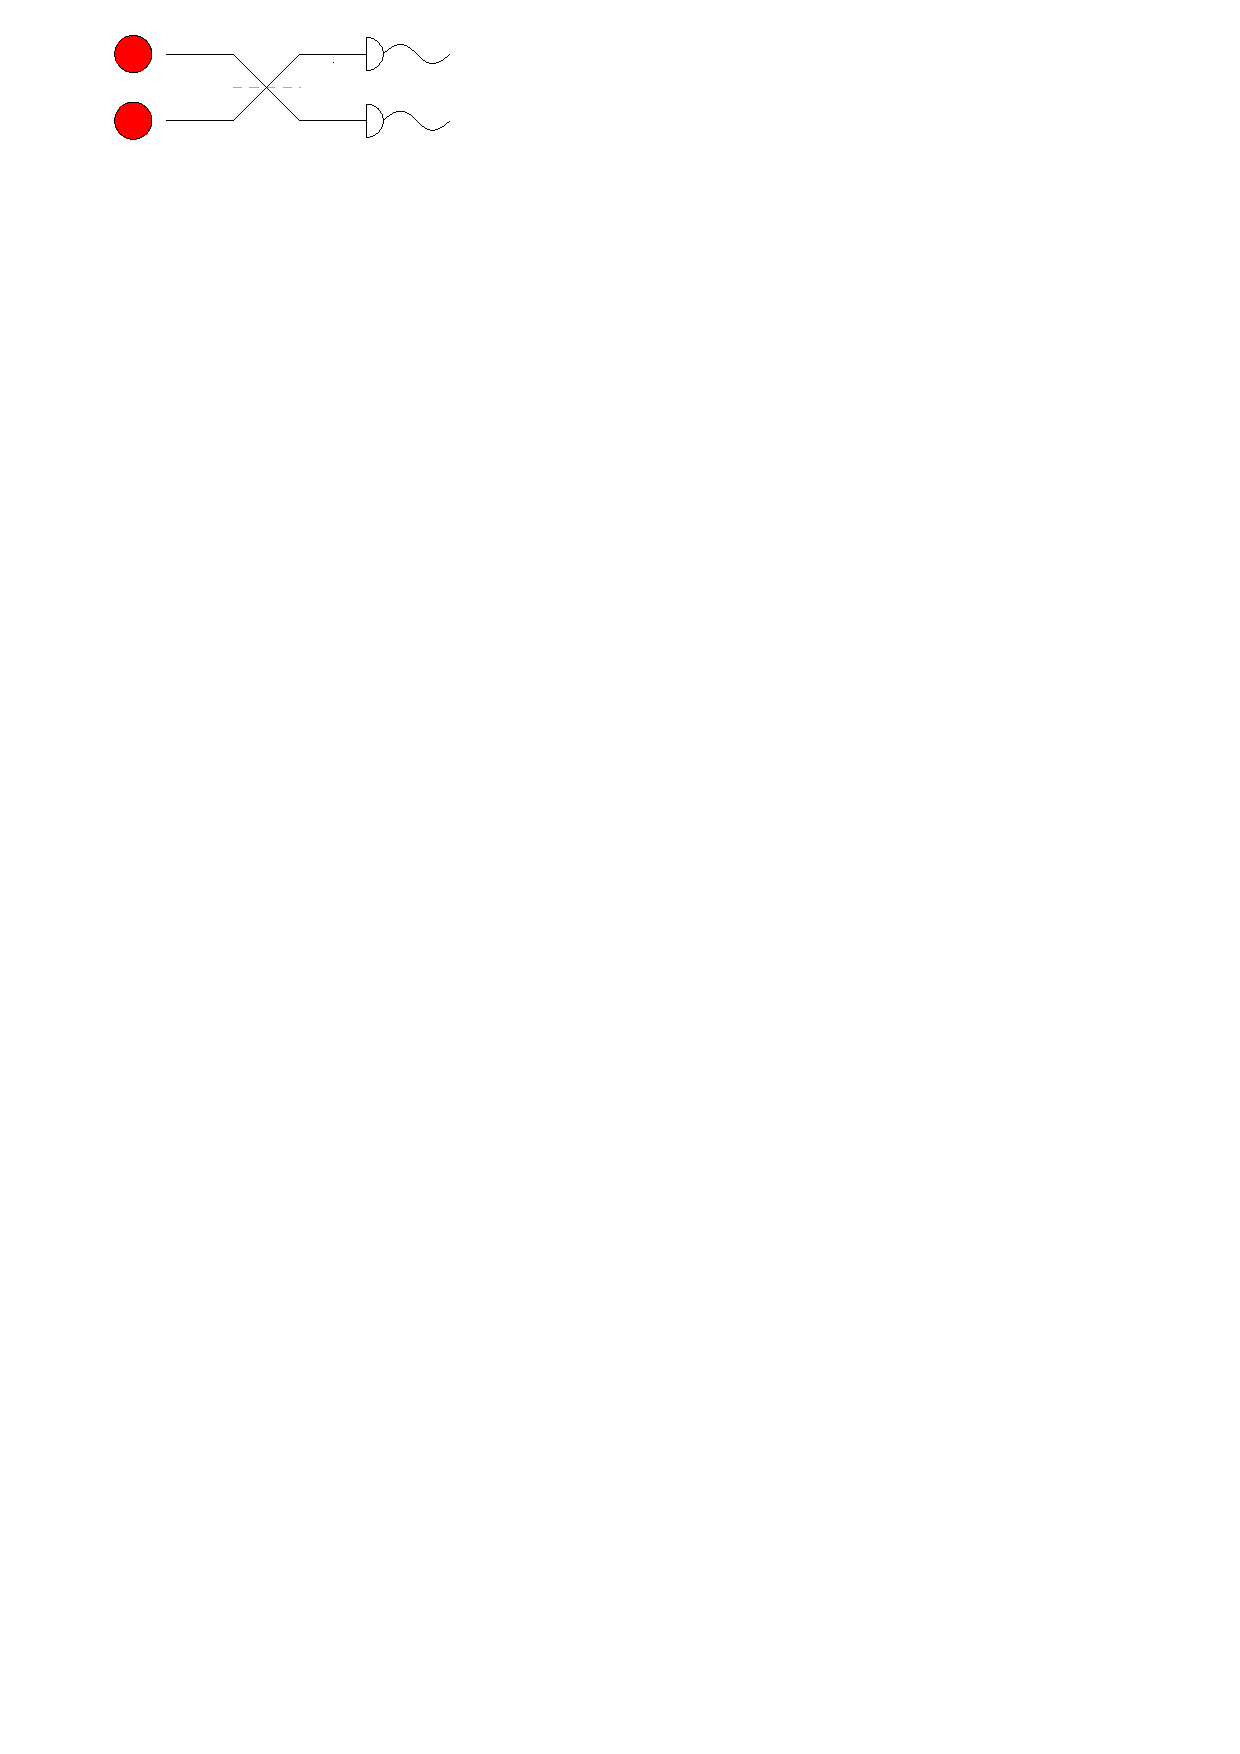
\includegraphics[width=0.45\linewidth]{preliminary_bs/hom}
\end{center}
\caption[Experimental setup of the Hong-Ou-Mandel Dip]{\label{fig:hom}An experimental diagram for the Hong-Ou-Mandel Dip, consisting of two indistinguishable photons (red circles) in two spatial modes (solid black lines) interacting with a single 50-50 beam splitter (grey dashed line) before being measured by single photon detectors (white semi-circles).}
\end{figure}

The Hong-Ou-Mandel (HOM) Dip is the earliest demonstration of multi-photon interference \cite{hong1987}. It features two spatial modes, each starting with a single photon, and consists of simply a 50-50 beam splitter across both modes.

In second quantisation, we start with the Fock state $\ket{1,1} = a_1^\dagger a_2^\dagger\ket{0,0}$. Applying the beam splitter gives us

\begin{align}
a_1^\dagger a_2^\dagger\ket{0,0} &\rightarrow \frac{1}{2}(a_1^\dagger+ia_2^\dagger)(ia_1^\dagger+a_2^\dagger)\ket{0,0}\\
&= \frac{1}{2}\left(i(a_1^\dagger)^2+a_1^\dagger a_2^\dagger-a_2^\dagger a_1^\dagger+i(a_2^\dagger)^2\right)\ket{0,0}\\
&= \frac{1}{2}\left(i(a_1^\dagger)^2+a_1^\dagger a_2^\dagger-a_1^\dagger a_2^\dagger+i(a_2^\dagger)^2\right)\ket{0,0}\\
&= \frac{i\left((a_1^\dagger)^2+(a_2^\dagger)^2\right)}{2}\ket{0,0}\\
&= \frac{i(\ket{2,0} + \ket{0,2})}{\sqrt{2}}.
\end{align}

After measurement, we will find that both photons will always be detected in the same (random) spatial mode. This example has a strong connection to distinguishability, and we will return to it in Section \ref{ssec:imperfections-distinguishability}.

In first quantisation, we start with the state $(\ket{12} + \ket{21})/\sqrt{2}$. The beam splitter acts on each particle individually, giving

\begin{align}
\ket{\psi} &= \frac{1}{2\sqrt{2}}\left(\left(\ket{1} + i\ket{2}\right)\left(i\ket{1} + \ket{2}\right) + \left(i\ket{1} + \ket{2}\right)\left(\ket{1} + i\ket{2}\right)\right)\\
&= \frac{1}{2\sqrt{2}}\left(2i\ket{11} + (1+i^2)\ket{12} + (i^2+1)\ket{21} + 2i\ket{22}\right)\\
&= \frac{i(\ket{11}+\ket{22})}{\sqrt{2}}.
\end{align}

Again, we find that only bunching is observed at the output.

\subsection{Bosonic sampling}
\label{ssec:bosonic-sampling}

We now define the ideal probability distribution of indistinguishable single bosons interacting on a linear interferometer.
We'll refer to this as bosonic sampling, as it's a bit more general than Aaronson and Arkhipov's Boson Sampling problem as we describe below.
The input is $U \in \mathrm{U}(m)$, an $m\times m$ unitary matrix which describes an $m$-mode linear interferometer, and $S = (S_1,S_2,\dots,S_m)$ with $\sum_{i=1}^m S_i =n$, an ordered list of integers that corresponds to an $n$-boson, $m$-mode occupation describing the input state with $S_i$ bosons in mode $i$. 
Given an output occupation $S'$, define the $n \times n$ (not necessarily unitary) matrix $U_{S',S}$ as that formed by first taking $S_i'$ copies of row $i$ of $U$ in order to create an $m\times n$ matrix, from which we then take $S_j$ copies of column $j$. 
We can then define $\mathcal{D}_{U,S}$, the probability distribution for measuring an $n$-boson $m$-mode occupation $S'$ for interferometer $U$ and input state $S$, as
\begin{equation}\label{eqn:bs-distribution}
\textrm{Pr}_{\mathcal{D}_{U,S}}[S'] = \frac{|\per(U_{S',S})|^2}{\prod_{i=1}^m S_i'! S_i!} ,
\end{equation}
where $\per$ is the matrix permanent, defined as

\begin{equation}
\per(M) = \sum_{\sigma\in\symm_n}\prod_{i=0}^nM_{i,\sigma(i)}.
\label{eqn:permanent}
\end{equation}

This relationship between linear optics and matrix permanents was originally found by Scheel and Buhmann \cite{scheel2008}, and later proven by Aaronson and Arkhipov using a different approach \cite{aaronson2010report, aaronson2011}.

In a photonics experiment, this setting is described in terms of creation operators $a^\dag_i$ for a photon in mode $i$. 
The initial state is then
\begin{equation}
|S\rangle = \prod_{i=0}^m \frac{(a_i^\dagger)^{S_i}}{\prod_{j=2}^{S_i}\sqrt{j}}|0^m\rangle.
\end{equation}
The evolution of the photonic state induced by a linear optical interferometer implementing $U$ can then be expressed as $a_i^\dagger \mapsto \sum_{j = 0}^m U_{i,j}a_j^\dagger$.
Thus single boson states evolve under linear interferometry just as an $m$ dimensional qudit does under a unitary gate $U$ (sometimes called unary encoding).
This suggests how quantum circuits simulating photonics might be constructed, as we'll see.

The problem known as Boson Sampling is that of sampling from this probability distribution in the case where the input occupation is specified as $|1^n 0^{m - n}\rangle = \prod_{i = 1}^n a_{i}^\dagger|0\rangle$, and $U$ is drawn Haar randomly from U$(m)$ with $m=O(n^2)$\cite{aaronson2010report, aaronson2011}.

It is easy to see that both of the two examples discussed in Section \ref{ssec:example-interferometers} can be described in this picture as well. For the Mach-Zehnder Interferometer, we find that the unitary matrix describing our interferometer is

\begin{align}
U &= \frac{1}{2}\begin{pmatrix}1&i\\i&1\end{pmatrix}\begin{pmatrix}e^{i\theta}&0\\0&1\end{pmatrix}\begin{pmatrix}1&i\\i&1\end{pmatrix}\\
&= \frac{1}{2}\begin{pmatrix}e^{i\theta}&i\\ie^{i\theta}&1\end{pmatrix}\begin{pmatrix}1&i\\i&1\end{pmatrix}\\
&= \frac{1}{2}\begin{pmatrix}e^{i\theta}-1&i(e^{i\theta}+1)\\i(e^{i\theta}+1)&1-e^{i\theta}\end{pmatrix}.
\end{align}

Assuming our photon is initially in mode 1, the relevant matrices describing our outcomes are the $1\times 1$ matrices $M_{1,1} = e^{i\theta}-1$ and $M_{1,2} = i(e^{i\theta}+1)$. For $1\times 1$ matrices the permanent is just the single element, and so we find the probabilities are $|e^{i\theta}-1|^2$ and $|e^{i\theta}+1|^2$, giving us the expected outcome of controlling the photon output based on $\theta$.

For the Hong-Ou-Mandel Dip, we note that the relevant unitary matrix is the matrix we have for a beam splitter. We then note that the probability of seeing outcome occupation $\ket{1,1}$ is

\begin{align}
\left|\per\begin{pmatrix}\frac{1}{\sqrt{2}}&\frac{i}{\sqrt{2}}\\\frac{i}{\sqrt{2}}&\frac{1}{\sqrt{2}}\end{pmatrix}\right|^2 &= \frac{|1+i^2|^2}{4}\\
&= 0.
\end{align}

Similarly we find that the outcomes for $\ket{2,0}$ and $\ket{0,2}$ are

\begin{align}
\frac{\left|\per\begin{pmatrix}\frac{1}{\sqrt{2}}&\frac{i}{\sqrt{2}}\\\frac{1}{\sqrt{2}}&\frac{i}{\sqrt{2}}\end{pmatrix}\right|^2}{2!} &= \frac{|2i|^2}{8}\\
&= \frac{1}{2},
\end{align}

\noindent and

\begin{align}
\frac{\left|\per\begin{pmatrix}\frac{i}{\sqrt{2}}&\frac{1}{\sqrt{2}}\\\frac{i}{\sqrt{2}}&\frac{1}{\sqrt{2}}\end{pmatrix}\right|^2}{2!} &= \frac{|2i|^2}{8}\\
&= \frac{1}{2},
\end{align}

\noindent respectfully. This matches the expected outcome statistics of the coincident output never occurring and the two other possible outcomes happening purely at random.

\subsection{Universal linear optical interferometers}
\label{ssec:universal-lo}

\begin{figure}
\subfloat[\label{fig:reck}]{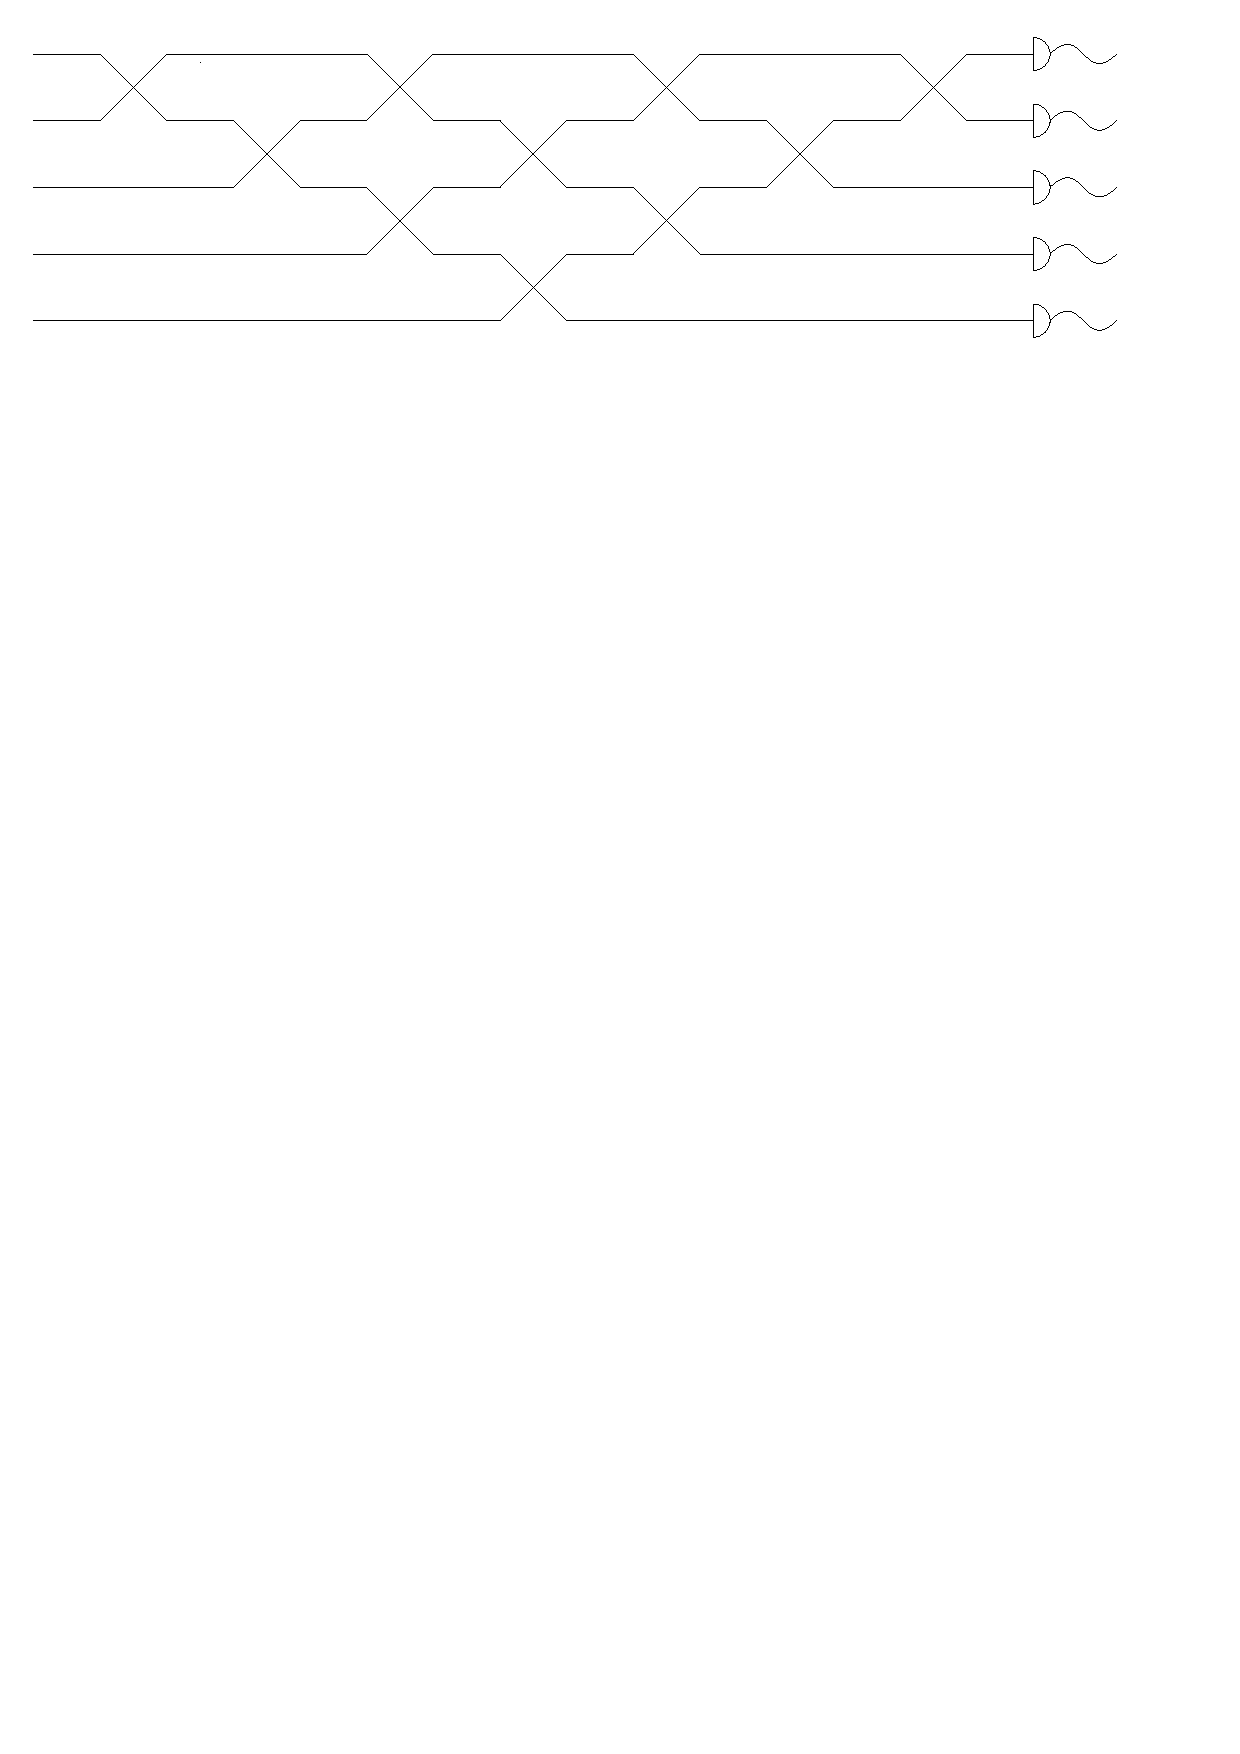
\includegraphics[width=0.45\linewidth]{preliminary_bs/reck}}
\hfill
\subfloat[\label{fig:clements}]{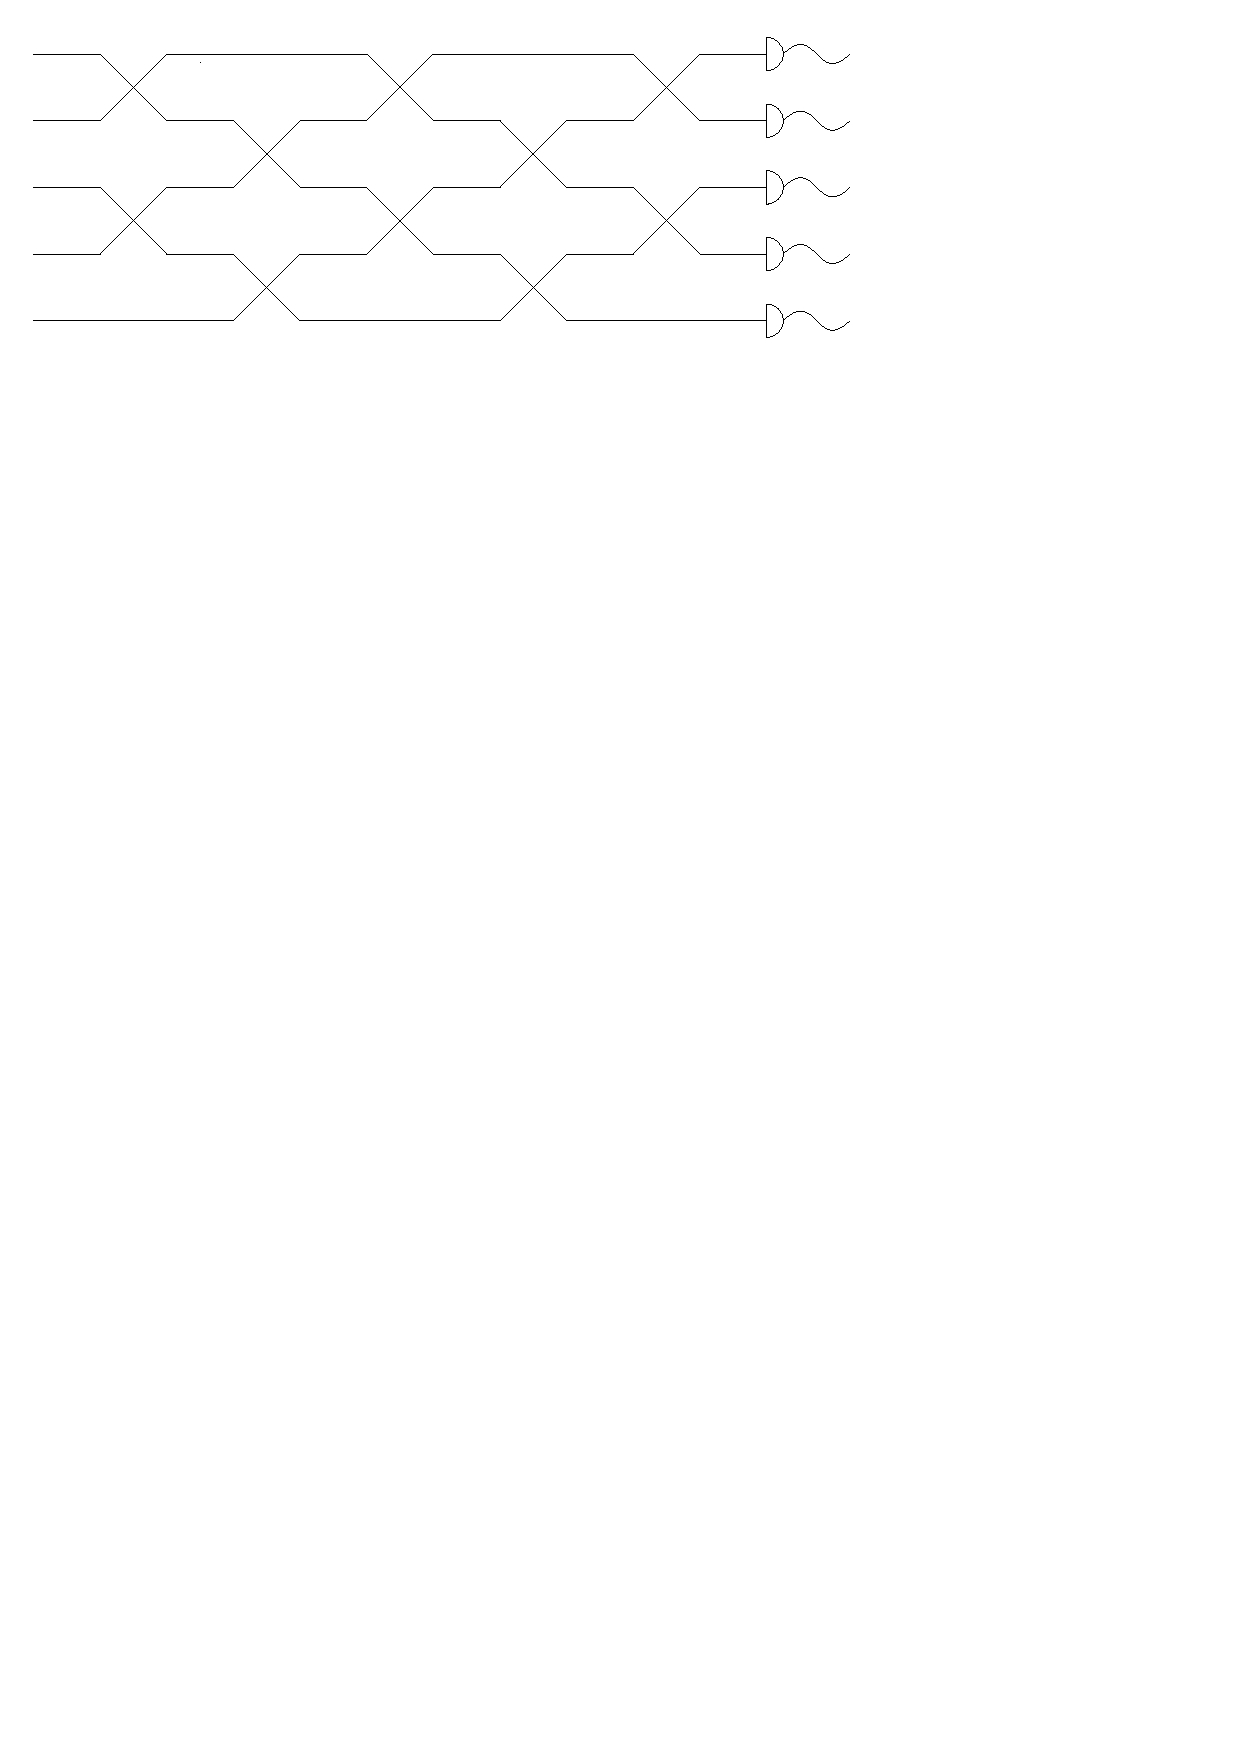
\includegraphics[width=0.45\linewidth]{preliminary_bs/clements}}
\caption[Two examples of universal linear-optical interferometers]{\label{fig:universal-lo}Two examples of universal linear-optical interferometers by (\ref{fig:reck}) Reck et al.~\cite{reck1994} and (\ref{fig:clements}) Clements et al.~\cite{clements2016}. Each point where two spatial modes overlap is a Mach-Zehnder interferometer, as described in Section \ref{ssec:example-interferometers}.}
\end{figure}

One of the requirements of Boson Sampling is that the unitary $U$ should be Haar-random. Choosing a unitary purely at random might seem like a challenge at first, but there are examples of linear optical interferometers which are fully reprogrammable. We will give two examples, from which any unitary can be implemented by reprogramming the phase shifters.

The first of these schemes was realised mathematically by Hurwitz, and later rediscovered by Reck et al.~\cite{hurwitz1897, reck1994}. This scheme uses a sequence of Mach-Zehnder interferometers arranged in a pyramid-like structure, shown in Figure \ref{fig:reck}. The universality of this scheme is proven recursively, by decomposing an $m\times m$ unitary matrix into an $(m-1)\times(m-1)$ unitary matrix accompanied by $m$ two-mode transformations in the $m$-th mode. These additional transformations can be implemented as Mach-Zehnder interferometers. However, a potential weakness with this interferometer is that it is of very high depth; a photon starting and finishing in mode 1 might interact with up to $2m-3$ beam splitters. This could result in experiments being impractically large, and also result in issues such as photon loss, something we will discuss further in Section \ref{ssec:imperfections-loss}.

These issues were addressed in a later interferometer designed by Clements et al.~\cite{clements2016}. This design is similarly constructed out of Mach-Zehnder interferometers, arranged in a chequerboard-like design alternating between pairs of modes, shown in Figure \ref{fig:clements}. The universality of this design is proven by decomposing the diagonals along either side of $U$ into two-mode transformations. This design has depth $m$, lower than that of the Hurwitz scheme above. It is also easy to see that a lower depth scheme is impossible, as a photon in mode 1 would then not be able to reach mode $m$.

\subsection{The computational complexity of Boson Sampling}
\label{ssec:cc-bs}

\begin{problem}[Boson Sampling] Let $U$ be an $m$-mode linear optical interferometer. Sample from the distribution corresponding to measuring $U$ acting on $|1^n0^{m-n}\rangle$ in the (anti-bunched) Fock basis, where $m=O(n^2)$.
\end{problem}

It was proven by Aaronson and Arkhipov that if there was a polynomial time classical algorithm for sampling from this distribution, then $\p^{\sharpp} = \bpp^{\np}$ and the Polynomial Hierarchy would collapse to the third level \cite{aaronson2010report, aaronson2011}. This is done using the fact that the permanent of a matrix is $\sharpp$-hard, even to approximate \cite{valiant1979, aaronson2011sharpp}. 
Aaronson and Arkhipov also showed the same result for sampling from any approximate distribution up to $\epsilon$ away in total variation distance from Boson Sampling, assuming the conjectures from before.

In comparison to the other quantum advantage problems, the anticoncentration conjecture has not been proven for Boson Sampling. It is also not known if it is $\sharpp$-hard to approximate the permanent of a random complex matrix, however it has been proven that exactly computing the permanent of a Gaussian matrix is $\sharpp$-hard \cite{aaronson2010report, aaronson2011}.

Regarding the question of verifying Boson Sampling, there have been some interesting results. Gogolin et al.~\cite{gogolin2013} argued that if a verifier does not know the underlying distribution, and is therefore only using the samples obtained to verify the distribution, then Boson Sampling requires an exponentially large number of samples to differentiate from the uniform distribution. This was refuted by Aaronson and Arkhipov \cite{aaronson2014}, who argued that this definition of a verifier is poor, akin to arguing that factoring an integer into its prime factors $N=pq$ should not be verified by multiplying $p$ and $q$ together, or that a Hamiltonian cycle in a graph shouldn't be verified by ensuring every vertex is visited exactly once. Aaronson and Arkhipov then develop further on this result, first showing that Boson Sampling is far from the uniform distribution in total variation distance, and then providing an explicit estimator which can discriminate Boson Sampling from the uniform distribution. But there are other classical distributions, notably Boson Sampling with fully distinguishable photons, which the algorithm fails to distinguish. This was resolved in work by Spagnolo et al.~\cite{spagnolo2014}, who experimentally implemented the uniform discriminator and developed another algorithm which could differentiate ideal Boson Sampling from Boson Sampling with fully distinguishable photons. Agresti et al.~\cite{agresti2019} later used the $K$-means clustering algorithm from machine learning, with a three-photon Boson Sampling experiment providing the target data, to discriminate between indistinguishable and distinguishable Boson Sampling as well. Agresti et al.\ then used classical Boson Sampling simulators (see Section \ref{sec:classical-simulations}) to test how effective their discriminator was using the same original test data to distinguish experiments with up to 25 photons across up to 625 modes, and found that in most cases $10^4$ samples were sufficient to distinguish the two distributions.

As we shall see in Section \ref{sec:experimental-achievements}, distinguishing from the two distributions above is a common technique for verifying Boson Sampling experiments today \cite{carolan2015, zhong2018, paesani2018, wang2019}. However, it is still unclear what properties can be used to fully distinguish Boson Sampling from other distributions which can be classically simulated. One proposal by Carolan et al.~\cite{carolan2014} was to use photon bunching to characterise effects, but this was quickly refuted by Tichy et al.~\cite{tichy2014}, who gave a Monte Carlo algorithm which could output a distribution with the same properties. Walschaers et al.~\cite{walschaers2016, walschaers2016thesis} later provided more refined statistical features from random matrix theory which can discriminate against all models discussed so far for $m<n^{5.1}$. Giordani et al.~\cite{giordani2018} demonstrate this experimentally, and use machine learning to identify what characteristics give way to these features. However, even with these approaches as $m$ and $n$ increase the distributions start to become more alike.

\subsection{Boson Sampling variants}
\label{ssec:bs-variants}

Since originally being proposed, a number of Boson Sampling variants have arisen to varying degrees of success, which aim to fix experimental challenges in vanilla Boson Sampling. We give two particular examples below which have been experimentally realised.

\begin{problem}[Scattershot Boson Sampling] Let $U$ be an $m$-mode linear optical interferometer. Sample from the distribution corresponding to measuring $U$ acting on $|\bar{S}\rangle$ in the (anti-bunched) Fock basis, where $m=O(n^2)$ and conditioned on sampling $\bar{S}$ uniformly at random from the $\binom{m}{n}$ ways of choosing $n$ out of $m$ input modes.
\end{problem}

One of the largest issues with Boson Sampling is generating the input state $\ket{1^n0^{m-n}}$. This is because we do not currently have deterministic single photon sources. If a single photon source outputs a photon with probability $p$, $n$ independent sources will all generate single photons with probability $p^n$, so we will have to wait an exponentially long time just to generate enough photons.

The idea of Scattershot Boson Sampling is to increase the number of probabilistic photon sources and condition the distribution on which sources output a photon \cite{aaronson2013, lund2014}. This can be implemented experimentally by using heralded sources, which use nonlinear optical effects such as Spontaneous Parametric Down Conversion to generate a pair of photons of different wavelengths \cite{loudon2006}. By measuring one of these photons, we know that a pair of photons were generated in this spatial mode and therefore we can input the other photon to our interferometer. Now if there are $n$ heralded sources each firing with probability $p$, then we expect on average $np$ photons to be input to our interferometer.

It is worth noting that with heralded photon sources there is also a probability that more than one pair of photons is generated by a single source. Although it is not fully clear how the computational hardness is affected when multiple photons are generated in the same mode, it is known that photons generated in the same spatial mode do not interfere with each other. We can avoid this scenario by limiting the probability of a successful herald. Christ and Silberhorn estimate that a heralding probability of $25\%$ is optimal for achieving the best success rate while also minimising multi-photon emissions, and recommend active switching to improve heralding rates even further \cite{christ2012}.

\begin{problem}[Gaussian Boson Sampling] Let $U$ be an $m$-mode linear optical interferometer. Sample from the distribution corresponding to measuring $U$ acting on $|\zeta^n0^{m-n}\rangle$ in the (anti-bunched) Fock basis, where $m=O(n^2)$ and $|\zeta\rangle$ is a single mode squeezed vacuum state.
\end{problem}

Gaussian Boson Sampling is another proposed way of working around the need for single photon sources \cite{hamilton2017}. The idea is to start with $k\approx n$ single mode squeezed states, each generated from the $\ket{0}$ Fock state. These squeezed states are then input into an interferometer and measured in the Fock basis.

Hamilton et al.~\cite{hamilton2017} used arguments akin to Aaronson and Arkhipov to argue that Gaussian Boson Sampling is computationally hard. The main difference between the two is that the probability of a particular output from Gaussian Boson Sampling is proportional to another $\sharpp$-Hard function called the Hafnian of a $2n\times 2n$ matrix, rather than the permanent of an $n\times n$ matrix. From this starting point the rest of the argument follows through. Another intuitive way of seeing this is in Aaronson, courtesy of Garc\'{i}a-Patr\'{o}n \cite{aaronson2013}, by noting that Scattershot Boson Sampling can be reduced to Gaussian Boson Sampling. To do this, we simply embed the photon pair sources into the Gaussian Boson Sampling experiment by generating two-mode entangled squeezed states and using them as input.

Another unexpected benefit of Gaussian Boson Sampling is that there are some applications demonstrated. Huh, et al.~\cite{huh2015} showed that Gaussian Boson Sampling could be used to simulate the vibronic spectra of molecules. It has also recently been shown by Bradler et al.\ and Schuld et al.\ at Xanadu that graphs can be encoded into Gaussian Boson Sampling experiments in a way such that different graphs provide different measurement statistics, thus giving a way of solving the Graph Isomorphism problem \cite{bradler2018, schuld2019}.

It is worth noting that measuring in the Fock basis is crucial for computational hardness in Gaussian Boson Sampling. In particular, if the measurement is instead a Homodyne measurement for measuring Gaussian states, the resulting distribution is classically simulable in polynomial time \cite{bartlett2003}.

\section{Experimental Achievements}
\label{sec:experimental-achievements}

Since originally being proposed in 2010, Boson Sampling has taken the interest of a number of quantum optics research groups, each eager to demonstrate a quantum advantage through this process. We provide some of the results of said groups below.

The earliest experimental demonstrations were shown in 2013, by four different groups independently \cite{broome2013, spring2013, tillmann2013, crespi2013}. These results were published simultaneously, with two publications in \emph{Nature Photonics} and two in \emph{Science}. All four results used reprogrammable designs on integrated photonic circuits to implement the unitary transformation. Crespi et al.~\cite{crespi2013} and Tillmann et al.~\cite{tillmann2013} both demonstrated Boson Sampling with up to three photons across five modes. Broome et al.~\cite{broome2013} demonstrated three photons across six spatial modes, while Spring et al.~\cite{spring2013} demonstrated four photons across six modes. Crespi et al., Broome et al., and Spring et al., verified their experimental results by computing the distance between their experimental distribution and the theoretical distribution \cite{spring2013, tillmann2013, crespi2013}, while Tillman et al.\ verified their experiment by estimating the fidelity \cite{tillmann2013}.

Later in 2015, an experiment by Carolan et al.~\cite{carolan2015} demonstrated experimental Boson Sampling with six photons across six modes. This was implemented on a fully reprogrammable integrated silica circuit. One caveat is that the authors used the input Fock state $\ket{3,3,0,0,0,0}$, rather than the traditional form of having single photons in each mode. The authors justify this in order to use the verification approach of \cite{carolan2014}, though as discussed in Section \ref{ssec:cc-bs} this verification approach has limitations of its own. This device was later also used by Sparrow, Mart\'{i}n-L\'{o}pez et al.~\cite{sparrow2018} with two-mode squeezed inputs and adaptive feedback to simulate the vibronic structure of a variety of 4-atom molecules, hinting at a potential application for bosonic sampling.

The first Boson Sampling demonstration with five single photons was performed in 2017 by Wang et al.~\cite{wang2017}. Wang et al.\ used a triangular array of beam splitters bonded together to create a structure smaller than regular bulk optics but larger than integrated silicon or silica chips, featuring 9 input and output modes. Wang et al.\ state that many interferometers can be generated from this chip by adjusting the polarisation of photons, but acknowledge that the structure itself is not universal. Boson Sampling is verified in this experiment by checking against the uniform and fully distinguishable distributions.

Following this came a few results on up to five photons for Boson Sampling variants. Zhong et al.~\cite{zhong2018} demonstrated Scattershot Boson Sampling with up to five photons across twelve modes, using an interferometer constructed by six trapezoidal quartz blocks covered in film and fused together. Then, Paesani et al.~\cite{paesani2018} demonstrated four photon Scattershot, Gaussian and vanilla Boson Sampling on a single integrated silicon chip, by simply adjusting which state they input to the chip. Finally, Zhong et al.~\cite{zhong2019} demonstrated Gaussian Boson Sampling with up to five photons, using the same interferometer as in \cite{zhong2018}. All of the standard and Scattershot Boson Sampling experiments were validated by comparison to distinguishable and uniform sampling. In the case of Gaussian Boson Sampling, comparisons were also made to thermal states, non-squeezed coherent states and two-mode squeezed states, as well as demonstrating applications related to molecular simulations and graph theory \cite{paesani2018, zhong2019}.

The most recent experimental demonstration of Boson Sampling was performed in 2019 by Wang et al.~\cite{wang2019}. This experiment used a 3D integrated photonic circuit with 60 spatial modes. Wang et al.\ managed to demonstrate standard Boson Sampling with up to 10 photons, as well as Boson Sampling under loss with up to 20 input photons and 14 output photons, both of which were verified by comparison to uniform and distinguishable photon distributions. To date this is the largest demonstration of Boson Sampling publicly announced.

\section{Experimental Imperfections in Linear Optics}
\label{sec:lo-imperfections}

We shall now discuss two imperfections that are particularly common in Boson Sampling. The first is distinguishability, when one or more factors make bosons distinct from one another. The second, loss, is when photons which are generated at input are not detected at the output. We shall discuss some ways in which these issues occur, how they affect the probability distributions, and what is known about their computational complexity. In Section \ref{sec:classical-simulations}, we shall discuss some of the classical simulation algorithms that have been developed surrounding these issues.

\subsection{Distinguishability}
\label{ssec:imperfections-distinguishability}

One of the points made when discussing Boson Sampling is that the photons need to be indistinguishable. This means that if we permuted the photons in some way, it would be impossible for someone else to identify which permutation was applied.

A number of internal characteristics about the photons could make them distinguishable. The most visually intuitive one is wavelength: A red photon is definitely distinct from a green photon. But other aspects could also distinguish photons, such as their polarisation, or what time they were generated. The time generation point is particularly important following the discussion in Section \ref{ssec:bs-variants} about the challenges of single photon sources: Not only do all of these single photon sources need to emit a photon, but all of them need to emit photons at the exact same time. We can model distinguishability by introducing additional modes to describe the internal state. Throughout this thesis, we will use spatial or ``system'' modes to describe where a photon is, and internal or ``label'' modes to describe its distinguishable characteristics.

Before we consider Boson Sampling with distinguishability, we will first return to the Hong-Ou-Mandel dip from Section \ref{ssec:example-interferometers} \cite{hong1987}. This time, we will consider one red photon generated in mode $1$, and one photon generated in mode 2 which is red with amplitude $v\in [0,1]$ and green with amplitude $d=\pm\sqrt{1-v^2}$. We can represent this in second quantisation by introducing additional indices to our creation and annihilation operators: $a_{i,R}^\dagger$ and $a_{i,G}^\dagger$ to indicate a red or green photon in mode $i$, respectively. Our input is now

\begin{equation}
a_{1,R}^\dagger\left(v a_{2,R}^\dagger + da_{2,G}^\dagger\right)\ket{0_R,0_G,0_R,0_G}.
\end{equation}

After applying the beam splitter our photons are in the state

\begin{align}
a_{1,R}^\dagger\left(v a_{2,R}^\dagger + da_{2,G}^\dagger\right)\ket{0_R,0_G,0_R,0_G} &\rightarrow \frac{1}{2}\left(a_{1,R}^\dagger + ia_{2,R}^\dagger\right)\nonumber\\
&\times\left(v\left(ia_{1,R}^\dagger + a_{2,R}^\dagger\right) + d\left(ia_{1,G}^\dagger + a_{2,G}^\dagger\right)\right)\ket{0_R,0_G,0_R,0_G}\\
&= \frac{v}{2}\left(i(a_{1,R}^\dagger)^2 + a_{1,R}^\dagger a_{2,R}^\dagger - a_{2,R}^\dagger a_{1,R}^\dagger+i(a_{2,R}^\dagger)^2\right)\nonumber\\
&\times\ket{0_R,0_G,0_R,0_G}\nonumber\\
&+\frac{d}{2}\left(ia_{1,R}^\dagger a_{1,G}^\dagger + a_{1,R}^\dagger a_{2,G}^\dagger - a_{2,R}^\dagger a_{1,G}^\dagger+ia_{2,R}^\dagger a_{2,G}^\dagger \right)\nonumber\\
&\times\ket{0_R,0_G,0_R,0_G}\nonumber\\
&= \frac{v}{2}\left(i(a_{1,R}^\dagger)^2 +i(a_{2,R}^\dagger)^2\right)\ket{0_R,0_G,0_R,0_G}\nonumber\\
&+\frac{d}{2}\left(ia_{1,R}^\dagger a_{1,G}^\dagger + a_{1,R}^\dagger a_{2,G}^\dagger - a_{2,R}^\dagger a_{1,G}^\dagger+ia_{2,R}^\dagger a_{2,G}^\dagger \right)\nonumber\\
&\times\ket{0_R,0_G,0_R,0_G}\nonumber\\
&= \frac{v}{2}\left(i(a_{1,R}^\dagger)^2 +i(a_{2,R}^\dagger)^2\right)\ket{0_R,0_G,0_R,0_G}\nonumber\\
&+\frac{d}{2}\left(ia_{1,R}^\dagger a_{1,G}^\dagger + a_{1,R}^\dagger a_{2,G}^\dagger - a_{2,R}^\dagger a_{1,G}^\dagger+ia_{2,R}^\dagger a_{2,G}^\dagger \right)\nonumber\\
&\times\ket{0_R,0_G,0_R,0_G}\\.
\end{align}

Note that in the final line, the terms $a_{1,R}^\dagger a_{2,G}^\dagger$ and $a_{2,R}^\dagger a_{1,G}^\dagger$ do not cancel out, due to the different creation operators from the fact that the photons are different colours. We apply our creation operators to reach the final state

\begin{align}
&\frac{1}{2}\left(v\left(i\sqrt{2}\ket{2_R,0_G,0_R,0_G} +i\sqrt{2}\ket{0_R,0_G,2_R,0_G}\right)\right)\nonumber\\
&+\frac{1}{2}\left( d\left(i\ket{1_R,1_G,0_R,0_G} + \ket{1_R,0_G,0_R,1_G} - \ket{0_R,1_G,1_R,0_G}+i\ket{0_R,0_G,1_R,1_G} \right)\right).
\end{align}

\begin{figure}
\begin{center}
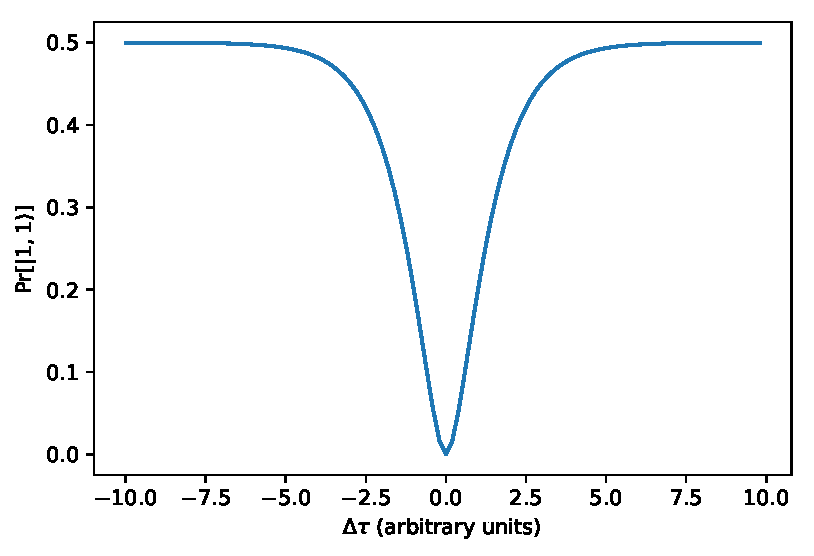
\includegraphics[width=0.5\linewidth]{preliminary_bs/hom_plot}
\end{center}
\caption{\label{fig:hom-plot}The probability of seeing the coincident $\ket{1,1}$ output from a Hong-Ou-Mandel experiment over $\Delta\tau$.}
\end{figure}

If we only measure what spatial mode our photons are in and discard the wavelength, we will find that we are in the Fock state $\ket{2,0}$ with probability $v^2/2 + d^2/4$ and likewise for $\ket{0,2}$, but we'll also find ourselves in the state $\ket{1,1}$ with probability $d^2/2$. Noting that $d^2 = 1-v^2$ and that $v=e^{-\Delta\tau}$ for some $\Delta\tau\in \mathbb{R}$ such that $\Delta\tau \geq 0$, it is easy to see that adjusting $\Delta\tau$ determines how likely we are to see coincidences at the output: if $\Delta\tau=0$, meaning that our photons are completely indistinguishable, we don't see any coincidences at all; as $\Delta\tau\rightarrow\pm\infty$, corresponding to completely distinguishable photons, then we see coincidences with probability 1/2. This is where the ``dip'' in Hong-Ou-Mandel Dip comes from: as our photons become more indistinguishable we see a drop in coincidences. This is plotted visually in Figure \ref{fig:hom-plot}. The extent to which we see a dip is known as the visibility of a Hong-Ou-Mandel dip, hence $v$, and is a standard technique when characterising linear optics experiments to determine how distinguishable pairs of photons are. Physically, $\Delta\tau$ corresponds to the difference between our photons, for example if there is a difference in path length between the photon sources and the beamsplitter.

In first quantisation, we can likewise realise this interference by introducing a second register noting what label mode our photons are in. Our state is now

\begin{equation}
\ket{\psi} = \frac{1}{\sqrt{2}}\left(v(\ket{12}+\ket{21})\ket{RR}+d(\ket{12}\ket{RG} + \ket{21}\ket{GR})\right).
\end{equation}

Our unitary $U$ will act as $U\otimes U$ on the spatial modes and $I\otimes I$ on the label modes. Thus, our state evolves to

\begin{align}
U^{\otimes 2}\otimes I^{\otimes 2}\ket{\psi} &= \frac{v}{2\sqrt{2}}\left((2i\ket{11}+(1+i^2)\ket{12}+(i^2+1)\ket{21}+2i\ket{22})\ket{RR}\right)\nonumber\\
&+\frac{d}{2\sqrt{2}}\left(i\ket{11}(\ket{RG}+\ket{GR})+i\ket{22}(\ket{RG}+\ket{GR})\right)\nonumber\\
&+\frac{d}{2\sqrt{2}}\left(\ket{12}(\ket{RG}-\ket{GR})+\ket{21}(\ket{GR}-\ket{RG})\right)\\
&= \frac{iv}{\sqrt{2}}\left((\ket{11}+\ket{22})\ket{RR}\right)\nonumber\\
&+\frac{d}{2\sqrt{2}}\left(i(\ket{11}+\ket{22})(\ket{RG}+\ket{GR})+(\ket{12}-\ket{21})(\ket{RG}-\ket{GR})\right).
\end{align}

Again, we see that coincidences occur with probability $d^2/2$, matching the first quantisation result.

A rich library of theoretical work has been developed on the topic of Boson Sampling under distinguishability in recent years \cite{rohde2015, shchesnovich2015, tichy2015, tamma2016nonidentical, menssen2017}. Here, we shall follow the notation of Tichy \cite{tichy2015}, but note that this model of distinguishability is equivalent to several of the other models also mentioned. Tichy uses an $m\times m$ Gram matrix $\mathcal{S}_{i,j}$ to discribe the indistinguishability between photons generated in mode $i$ and photons generated in mode $j$, noting that any pair of photons generated in the same mode are indistinguishable from one another. Under Tichy's model, the probability of outcome $\ket{S'}$ is

\begin{equation}
\prob[S'] = \sum_{\sigma\in\symm_n}\prod_{i=1}^n\mathcal{S}_{i,\sigma(i)}\per(U_{S',S}*U_{S',\sigma(S)}^*),
\label{eqn:tichy-perm}
\end{equation}

\noindent where $*$ denotes element-wise multiplication, $M^*$ is the matrix whose elements are complex conjugates of $M$, and $\sigma(S)$ means the elements of $S$ permuted by $\sigma$. Again, the Hong-Ou-Mandel Dip can be visualised in this instance by noting that $\mathcal{S}_{1,2} = \mathcal{S}_{2,1} = v$:

\begin{align}
\prob[(1,1)] &= \per\begin{pmatrix}\frac{1}{\sqrt{2}}\times\frac{1}{\sqrt{2}}&\frac{i}{\sqrt{2}}\times\frac{-i}{\sqrt{2}}\\\frac{i}{\sqrt{2}}\times\frac{-i}{\sqrt{2}}&\frac{1}{\sqrt{2}}\times\frac{1}{\sqrt{2}}\end{pmatrix} + v^2 \per\begin{pmatrix}\frac{1}{\sqrt{2}}\times\frac{-i}{\sqrt{2}}&\frac{i}{\sqrt{2}}\times\frac{1}{\sqrt{2}}\\\frac{i}{\sqrt{2}}\times\frac{1}{\sqrt{2}}&\frac{1}{\sqrt{2}}\times\frac{-i}{\sqrt{2}}\end{pmatrix}\\
&= \per\begin{pmatrix}\frac{1}{2}&\frac{1}{2}\\\frac{1}{2}&\frac{1}{2}\end{pmatrix} + v^2 \per\begin{pmatrix}\frac{-i}{2}&\frac{i}{2}\\\frac{i}{2}&\frac{-i}{2}\end{pmatrix}\\
&= \frac{2-2v^2}{4}\\
&= \frac{1-v^2}{2}\\
&= \frac{d^2}{2},
\end{align}

\noindent matching the result discussed above.

So what can be done to work around distinguishability? A few options are available. Shchesnovich used average mutual fidelity to give an upper bound on the complexity, stating that a sampling experiment is more powerful when the single-photon mode mismatch scales as $O(n^{-3/2})$ for $n$ photons~\cite{shchesnovich2014}. Rohde and Ralph \cite{rohde2012} suggest applying filtering to discard photons which are too distinguishable. This does end up creating loss as a result, trading one imperfection for another, but this can be tolerable to some extent, as we shall see in Section \ref{ssec:imperfections-loss} \cite{rohde2012, aaronson2016}. Another option, known as Multi-Boson Correlation Sampling \cite{tamma2014, tamma2015, laibacher2015, tamma2016, laibacher2017}, is to measure across some of these characteristics in such a way that the photons end up essentially behaving indistinguishably. Laibacher and Tamma used an example where $n$ photons were of different colours, and showed that a suitable time interval and polarisation could be chosen such that at the detectors the photons appeared indistinguishable. This was later demonstrated experimentally by Wang et al.~\cite{wang2018timebin}, as well as a subsequent experiment by Orre et al.~\cite{orre2019} where frequency-resolving detectors were used to demonstrate Boson Sampling with photons generated at different time.

Finally, we note there are a number of results that link distinguishability in linear optics to representation theory \cite{adamson2008, deguise2014, turner2016, menssen2017, stanisic2018}. We will introduce representation theory in Section \ref{sec:sw-duality}, and explain its link to Boson Sampling in more detail in Chapter \ref{chp:noisy_circuit}.

\subsection{Loss}
\label{ssec:imperfections-loss}

We now turn to photon loss, where we know that some photons were generated at the input but not detected at the output. There are a wide variety of reasons for why this might occur, including coupling between optical components, two-photon absorption, Rayleigh scattering and detector inefficiencies.

Consider a Boson Sampling experiment which starts with $n$ photons, of which only $k$ are detected. Crucially, not only does loss reduce the number of photons, but also we do not know which of the photons have been lost. This leads to the probability distribution forming a convex sum over different subsets of input photons

\begin{equation}
\prob[K'] = \sum_{\substack{K \subseteq S\\|K| = k}}p_{K}|\per(U_{K',K})|^2,
\end{equation}

\noindent where $p_K$ is the probability of the photons which started in input modes $K$ surviving, with $\sum_Kp_K = 1$.

One known complexity result is by Aaronson and Brod \cite{aaronson2016}, who considered Boson Sampling with uniform loss, meaning that $p_K=1/\binom{n}{k}\forall K$. Aaronson and Brod showed that in this model, Boson Sampling remains classically hard if $k=n-\ell$ for some constant $\ell$. This was proven by showing that if someone could estimate a convex sum of squared permanents of submatrices of an $(n)\times(n)$ matrix, then one can estimate the squared permanent of an $(n-\ell)\times(n-\ell)$ matrix with bounded probability. However, this only works if a constant number of photons are lost, regardless of how large $n$ is. No hardness proofs exist even for the case of a constant fraction of photons being lost.

Two papers have experimentally explored Boson Sampling under loss. The first, in 2018 by Wang et al.~\cite{wang2018}, considers five, six and seven photon Boson Sampling with one and two photons lost. The second, as mentioned in Section \ref{sec:experimental-achievements}, was performed in 2019 by Wang et al.~\cite{wang2019}, and demonstrates Boson Sampling with 20 input photons of which up to 14 survive.

\subsection{Other Imperfections}

Before we move on to classical simulations, we will briefly mention here other imperfections that might occur or be considered in a Boson Sampling experiment, as well as what results are known for these models.

\subsubsection{Low depth interferometers}

Loss is more likely to occur in Boson Sampling if the interferometer has a high depth. An intuitive question to ask in this case is what can be done with a Boson Sampling circuit of reduced depth? A hardness proof for exact sampling was given Brod \cite{brod2015}, showing that even four layers of beam splitters was sufficient to ensure hardness in the exact case. Classical algorithms for these instances were later devised, by taking advantage of the low depth to only simulate interference between photons which could actually cross paths \cite{deshpande2018, maskara2019}. Note that these classical simulation algorithms inherently assume the photons are not all generated adjacently from each other.

\subsubsection{Dark counts and Gaussian noise}

Dark counts occur when a detector registers a photon even though one was not present. This is most often due to thermal noise within the single photon detector, meaning that even if the detector was in complete darkness it would still claim that photons were present.

Dark counts themselves are not much of a challenge in Boson Sampling experiments; superconducting nanowire single photon detectors have sufficiently low dark counts that false clicks can be noticed easily and the experiment discarded \cite{kitaygorsky2005}. However, where they become challenging is when loss is also involved: It is very difficult to differentiate between a photon not being lost and a photon being lost combined with a false click at the detector. Shchesnovich \cite{shchesnovich2019} argued that this is akin to a model of Boson Sampling by Kalai and Kindler \cite{kalai2014}. Under Kalai and Kindler, Boson Sampling experiences a model of noise where the probability is still related to the permanent of a matrix, but now  the matrix in question is $\sqrt{1-\epsilon}U_{S',S}+\sqrt{\epsilon}X$ for some Gaussian matrix $X$ that acts as our noise. Kalai and Kindler suggest that for $\epsilon=\omega(1/n)$, vanilla Boson Sampling and Boson Sampling under Gaussian noise are already uncorrelated, and furthermore for $\epsilon = \Omega(1)$, that the probability of an outcome of Boson Sampling under Gaussian noise can be approximated by up to constant error. Shchesnovich \cite{shchesnovich2019} uses this result to propose a classical simulation algorithm, using techniques similar to those used for classically simulating Boson Sampling under distinguishability \cite{renema2018, renema2018loss}, which we shall explore further in Section \ref{sec:renema-review}.

\section{Classical Simulation Algorithms}
\label{sec:classical-simulations}

Having introduced distinguishability and loss, we are now ready to discuss classical simulation algorithms for these imperfections. We will start by explaining classical algorithms for vanilla Boson Sampling, which were the original classical simulators devised. We will then discuss Boson Sampling under fully distinguishable photons, as well as Boson Sampling under various models of loss. Finally, we shall consider the classical simulation algorithms of \cite{renema2018, renema2018loss}, which were the first known classical algorithms to consider both distinguishability and loss.

\subsection{Simulation algorithms for ideal Boson Sampling}

Boson Sampling under ideal conditions (lossless indistinguishable single photons) is intractable for sufficiently large $n$. 
Until recently the only classical simulation method explicitly known was to compute the entire probability distribution before taking a sample, though it was widely believed that more efficient, albeit still exponential time, approaches existed. 
A brute force method cannot scale, due to both the number of possible outcomes and the complexity of computing even one $n\times n$ complex matrix permanent.

Two major results gave the first explicit classical simulation strategies which were faster than brute-force sampling. 
The first, by Neville \textit{et al.}~\cite{neville2017}, demonstrated that Boson Sampling experiments with up to 30 photons could be simulated on a single laptop, and suggests that a supercomputer could handle up to 50 photons. 
This was achieved by starting with the classical distribution of $n$ distinguishable photons, and then using Metropolised Independence Sampling to adapt the distribution to that of ideal Boson Sampling.
The second result, by Clifford \& Clifford \cite{clifford2017}, gave a classical algorithm for exact Boson Sampling and runs in time equivalent to computing two $n \times n$ matrix  permanents per sample with a polynomial overhead. 
This is through a combination of optimizations, particularly computing marginal probabilities and sampling via the chain rule.
Our approach here is to make these more efficient techniques applicable to realistic situations with distinguishability and loss.

\subsection{A simulation algorithm for fully distinguishable Boson Sampling}
\label{ssec:fully-dist-sim}

In the case where the $n$ input photons are fully distinguishable, a simple polynomial time algorithm exists \cite{aaronson2014}. In this case, there is no photon interference, so photons can be sampled individually. This is done by taking a photon which starts in mode $i$, and sampling output mode $j$ with probability $|U_{j,i}|^2$. Repeating for all photons gives us the complete sample in $O(mn)$ time.

\subsection{Simulation algorithms for Boson Sampling with loss}

Another common source of imperfections in linear optics is that of photon loss, which arises through a number of different means. 
Indeed, any large-scale demonstration of Boson Sampling is bound to face photon loss, and therefore needs to take such issues into account. 
Some results have already shown instances where hardness is still retained, such as when only a constant number of photons are lost \cite{aaronson2016,wang2018}.

Neville \textit{et al.}\ compared the classical simulation of their approach to a Boson Sampling experiment where any photon loss was considered a rejected experiment \cite{neville2017}. Novel classical simulations for Boson Sampling under loss have also been considered by use of classically simulable states such as thermal \cite{garciapatron2017} or separable \cite{oszmaniec2018} states.

There has also been some consideration of how classical simulations can be generalised to non-uniform loss. 
This usually means photon loss that is dependent on the number of optical components, with each component having transmission probability $\tau$. 
Classical simulation methods can be generalised to this model by identifying a layer of uniform losses from the circuit, followed a non-uniform lossy circuit which can be simulated classically through the use of additional modes for lost photons \cite{garciapatron2017,oszmaniec2018}. 
These results showed that Boson Sampling under non-uniform loss can be classically simulated as long as the smallest number of components a photon encounters is logarithmic in $n$. More recently, methods were also developed to give a polynomial-time algorithm in the case where some photons experience little or no loss, by extracting losses into a layer of non-uniform loss and simulating via a generalisation of the Clifford \& Clifford algorithm \cite{brod2019}.

\subsection{Simulation under multiple imperfections}
\label{sec:renema-review}

In \cite{renema2018, renema2018loss}, Renema \textit{et al.}\ consider the Tichy model of inter-photon distinguishability described in Section \ref{ssec:imperfections-distinguishability}. 
The probability distribution of arbitrarily distinguishable bosons is modelled as
\begin{equation}
\prob[S'] = \sum_{\sigma\in\symm_n}\prod_{i=1}^n\mathcal{S}_{i,\sigma(i)}\per(M*M^*_{1,\sigma}) ,
\end{equation}
where $\mathcal{S}$ is the same matrix describing the distinguishability as in the previous section, $M$ is a matrix defined by the rows and columns of our interferometer $U$ selected based on our photon output $S'$ and input $S$, $M^*_{1,\sigma}$ is the conjugate matrix with the identity permutation applied to rows and permutation $\sigma$ applied to columns, and $*$ denotes element-wise multiplication. 
They further restrict to a model where the indistinguishability overlap is defined by a single parameter $\mathcal{S}_{i,j} = x + (1-x)\delta_{i,j}, x \in [0,1]$.
The sum over permutations can be ordered based on how many \emph{fixed points} a permutation has, giving
\begin{equation}
\prob[S'] = \sum_{j=0}^n\sum_{\sigma^j}x^j\per(M*M^*_{1,\sigma}) , \label{eqn:renema-state}
\end{equation}
where $\sigma^j$ denotes permutations which have $n-j$ elements as fixed points.
Each permanent can be broken down via the Laplace expansion into a sum of a complex matrix permanent multiplied by a positive matrix permanent:
\begin{equation}
\prob[S'] = \sum_{j=0}^n\sum_{\sigma^j}x^j\sum_{\substack{J'\leq S'\\|J'|=j}}\per(M_{J',1}*M^*_{J',\sigma_p})\per(|M_{\bar{J'},\sigma_u}|^2) ,
\end{equation}

\noindent where $J'$ is an occupation with $j$ photons. Here we are now choosing submatrices of $M$, with $J'$ representing the $\binom{n}{j}$ possible combinations of rows from $M$, $\bar{J'}$ representing the remaining rows, and $\sigma_p$ and $\sigma_u$  representing permuted and unpermuted elements of $\sigma$ respectively.
The $J' \leq S'$ notation is used to indicate that $J'$ is a Fock state such that $J_i\leq S'_i \,\forall i\in[m]$.

The classical simulation method used truncates the number of non-fixed points in a permutation as being at most $k$, with the remainder of the probability treated as an error margin. 
It is important to note while these approximations are real, they are not necessarily positive. 
This is due to the truncation, where positive higher order terms which would have corrected the probability to be positive are now missing from the approximation. 
To correct this, any negative approximations are rounded up to $0$.
These probabilities are then used to train a Metropolised Independence Sampler, akin to the technique of \cite{neville2017}. 
Training this sampler requires approximating a number of probabilities dependent on the underlying distribution, each of which involves computing $O(n^{2k})$ permanents of $k\times k$ complex matrices, and the same number of permanents of $(n-k)\times (n-k)$ matrices with non-negative entries. 
The permanents of $k\times k$ complex matrices can be computed classically in $O(k2^k)$ time via Ryser's algorithm, and the permanents of matrices with non-negative entries can be approximated up to multiplicative error in polynomial time \cite{jerrum2004,huber2008}. 
As long as $k$ is independent of $n$, this means that there is a polynomial runtime.

To work out a suitable value $k$, define coefficients $c_j$ as

\begin{equation}
c_j = \sum_{\sigma^j}\sum_{\substack{J'\leq S'\\|J'|=j}}\per(M_{J',1}*M^*_{J',\sigma_p})\per(|M_{\bar{J'},\sigma_u}|^2)\label{eqn:coefficients}.
\end{equation}

Assuming the matrices are Gaussian, the variance of each permanent can be bounded as

\begin{equation}
\var[\per(M_{J',1}*M^*_{J',\sigma_p})] = \frac{j!}{m^{2j}},
\end{equation}
and
\begin{equation}
\var[\per(|M_{\bar{J'},\sigma_u}|^2)] < \frac{(n-j)!}{m^{2(n-j)}}\sum_{l=0}^{n-j}\frac{1}{l!}.
\end{equation}

This leads to two key results. The first is that the variance of $c_j$ tends towards a constant value:
\begin{align}
\var[c_j] &< \left(\frac{n!}{m^n}\right)^2\frac{1}{e}\sum_{l=0}^{n-j}\frac{1}{l!} \label{eqn:var}\\
&\rightarrow\left(\frac{n!}{m^n}\right)^2 \textrm{ as } n\rightarrow\infty,
\end{align}
and the second is that the covariance for different values of $j$ is zero:
\begin{equation}
\cov[c_j,c_j'] = 0\, \forall\, j\neq j'\label{eqn:covar}.
\end{equation}
From this one can approximate the variance of the error as a geometric series, which as $n\rightarrow\infty$ tends towards the inequality
\begin{align}
\var[\Delta \prob[S']] &= \var[\prob[S']-\prob_k[S']]\\
&= \sum_{j=k+1}^nx^{2j}\var[c_j]\label{eqn:renema-variance}\\
&< \left(\frac{n!}{m^n}\right)^2\left(\frac{x^{2(k+1)}}{1-x^2}\right),
\end{align}
\noindent where $P_k$ is the probability distribution when truncated at $j\leq k$ for some $k<n$.

Finally one can use a Markov inequality to show that if the variance of the error is of the form $(n!/m^n)^2\epsilon^2$, the average error of the simulation is at most $\epsilon$ \cite{renema2018loss}.
Crucially, this value of $\epsilon$ is only dependent on $x$ and $k$ and no longer dependent on $n$.
This means that for any value of $x$, one can choose a suitable value of $k$ to achieve a required error $\epsilon$, and run a classical simulation in time polynomial in $n$.

In \cite{renema2018loss}, the method described above was adapted to consider uniform loss as well as distinguishability, showing that the same result can be found, with the only difference being that $x$ is now replaced by $\alpha=\sqrt{\eta}x$, where $\eta$ is the probability of each individual photon surviving. 
Crucially, this result demonstrated that Boson Sampling where a constant fraction of photons were lost can be simulated in $O(\ell^{2k}k2^k)$, where $\ell$ is the number of photons which survive and $k$ is only dependent on the constant $\ell/n$, distinguishability $x$, and the desired accuracy of the simulation. 
This can be expanded to classically simulating Boson Sampling under uniform loss by sampling $\ell$ from the binomial distribution before sampling output photons, which offers a runtime of $O(n^{2k}k2^k)$. 

Although this runtime is polynomial in terms of $n$ and can therefore be considered asymptotically efficient, it might not be classically simulable in practice. 
There are three main contributions to this: 
First, the algorithm is reliant on Metropolised Independence Sampling, which potentially requires many probabilities to be approximated per sample. 
Second, approximating each probability requires $O(n^{2k})$ permanents of $k\times k$ matrices, which even for small $k$ could be a large number of permanents. 
And third, approximating each probability requires $O(n^{2k})$ permanents of $(n-k)\times(n-k)$ matrices with non-negative elements. 
Although approximating permanents of matrices with non-negative elements can be achieved in polynomial time, classical algorithms still have a runtime ranging from $O((n-k)^4\log(n-k))$ to $O((n-k)^{7}\log^4(n-k))$, depending on the sparsity of the matrix~\cite{huber2008}. These issues are the main points to address in order to achieve a practical classical algorithm for Boson Sampling. The Clifford \& Clifford algorithm could help to alleviate these issues, but there is a challenge due to the fact that the approximation used in Renema et al.\ does not correspond to a bosonic state. 
This in turn leads to negative probabilities, which are not clear how to correct for in the Clifford \& Clifford algorithm.

\section{The Schur-Weyl Duality}
\label{sec:sw-duality}

We'll now turn to Schur-Weyl duality, a theorem related to the irreducible representations of the symmetric and unitary groups. Although this seems like a sudden jump in subject, we emphasise to the reader that the connection between linear optics and Boson Sampling as described earlier in this chapter and Schur-Weyl duality will be explained in Chapters \ref{chp:noisy_circuit} and \ref{chp:classical_sim}.

We will start by introducing representation theory, before explaining the Schur-Weyl duality in detail. At the end of this section we shall consider its connection to quantum information, and in Chapter \ref{chp:noisy_circuit} how it is linked to Boson Sampling specifically. For further reading we direct the reader to \cite{fulton2004, harrow2005}.

\subsection{Representation theory}

Let $G$ be a group and $X$ a set. We define an action of $G$ on $X$ as a map $\Phi\colon G\times X \rightarrow X$ such that the action of the identity element $e\in G$ is the identity map, $\Phi_e(x) = \Phi(e, x) = x$, and the following relation holds:

\begin{equation}
\Phi_{g_1}(\Phi_{g_2}(x)) = \Phi_{g_1g_2}(x).
\end{equation}

One trivial example is the action of the permutation group $S_n$ on the set of numbers from 1 to $n$, defined as $\Phi_\sigma(i) = \sigma(i)$. Note that $\Phi$ need not be injective with respect to $G$, so another trivial example is the identity action, which is $\Phi_g(x) = x \forall g \in G$.

A representation is defined as a vector space $V$ combined with an action $\Phi: G \times V \rightarrow V$ with the additional constraint that $\Phi$ is a linear map over $V$:

\begin{equation}
\Phi(g, u+v) = \Phi(g, u) + \Phi(g, v).
\end{equation}

Now let $W \subseteq V$ be a vector subspace. We say that $W$ is invariant with respect to the action of $\{\Phi_g\colon g\in G\}$ if

\begin{equation}
\Phi_g(w) \in W \forall g \in G, w \in W.
\end{equation}

Two trivial example of invariant subspaces are the full vector space $W=V$ and the empty vector space $W=\{0\}$. We call a vector subspace $W$ invariant if the above holds and $W$ is not equal to $V$ or $\{0\}$.

This finally brings us to the topic of irreducible representations. A representation $V, \Phi$ of $G$ is irreducible, also known as an irrep, if it contains no proper invariant subspaces. If $V$ does contain a proper invariant subspace, then we say that $V$ is reducible.

\subsection{Symmetric and Unitary Groups}

The main interest of this thesis is the representation theory of the unitary group U$(m)$, and their action on the space of $(\mathbb{C}^{m})^{\otimes n}$. The intuition for linking this to Boson Sampling is that each vector in $\mathbb{C}^m$ is referring to a photon which could be in one of $m$ modes, and the action of $U \in \unitary(m)$ will be our interferometer.
As we shall see, the irreducible representations for $\unitary(m)$ are intimately related to those of the symmetric group $\textrm{S}_n$.

For the tensor space of $(\mathbb{C}^{m})^{\otimes n}$, the actions of the symmetric and unitary groups on a tensor $v_1\otimes\dots\otimes v_n \in (\mathbb{C}^m)^{\otimes n}$ are explicitly as follows. 
For a permutation $\sigma \in \textrm{S}_n$, the action permutes the tensor factors,

\begin{equation}
\Phi_\sigma(v_1\otimes\dots\otimes v_n) = v_{\sigma^{-1}(1)}\otimes\dots\otimes v_{\sigma^{-1}(n)},
\end{equation}

\noindent and for a unitary matrix $U \in \textrm{U}(m)$, the action is the $n$-fold tensor product $\Phi_U = U^{\otimes n}$.

It is a simple exercise to see that these two actions commute:

\begin{align}
\Phi_U(\Phi_\sigma(v_1\otimes\dots\otimes v_n)) &= \Phi_U(v_{\sigma^{-1}(1)}\otimes\dots\otimes v_{\sigma^{-1}(n)})\\
&= (Uv_{\sigma^{-1}(1)})\otimes\dots\otimes(Uv_{\sigma^{-1}(n)})\\
&= \Phi_\sigma((Uv_1)\otimes\dots\otimes (Uv_n))\\
&= \Phi_\sigma(\Phi_U(v_1\otimes\dots\otimes v_n)).
\end{align}

The Schur-Weyl duality describes how $(\mathbb{C}^m)^{\otimes n}$ can be decomposed into irreps for the direct product group $\unitary(m)\times\symm_n$.

\begin{theorem}[Schur-Weyl duality~\cite{rowe2012}]
The complex vector space of $(\mathbb{C}^m)^{\otimes n}$ decomposes into irreducible subspaces
\begin{equation}
(\mathbb{C}^m)^{\otimes n} \simeq \bigoplus_{\lambda\vdash n} \mathbb{C}^{\{\lambda\}} \otimes \mathbb{C}^{(\lambda)} ,
\end{equation}
where $\mathbb{C}^{\{\lambda\}}$ carries irrep $\{\lambda\}$ of $\textrm{U}(m)$ and $\mathbb{C}^{(\lambda)}$ carries irrep $(\lambda)$ of $\textrm{S}_n$, and $\simeq$ indicates a change of basis is involved.
The dimension of irrep $(\lambda)$ can be viewed as the multiplicity of irrep $\{\lambda\}$, and vice versa.
\end{theorem}

It is common to label irreps of both of these groups by ordered partitions $\lambda = (\lambda_1,\lambda_2,\cdots,\lambda_m)$ of $n$ such that $\lambda_i \geq \lambda_{i+1}$ and $\sum_{i = 1}^m \lambda_i = n$.
We usually suppress zeros in this notation, so for example the totally symmetric irrep $\lambda=(n, 0,\dots,0)$ is written $(n)$. 
The number of nonzero $\lambda_i$ is called the length of the partition, $\ell(\lambda)$, and only partitions with $\ell(\lambda) \leq m$ occur, which we will assume in all of our expressions that follow. Similarly, the width of the partition is $w(\lambda) = \lambda_1$, the largest partition in $\lambda$.
%Following the convention of~\cite{rowe2012}, we shall label irreps of S$_n$ and U$(m)$ indexed by $\lambda$ as $(\lambda)$ and $\{\lambda\}$, respectively.

\subsection{The Quantum Schur Transform}

The Quantum Schur Transform realises the basis change of the Schur-Weyl Duality as a quantum circuit. This circuit takes as input a state in the basis $(\mathbb{C}^m)^{\otimes n}$, and decomposes it into a basis of states labelled by which irrep $\lambda$ they are in.

The canonical example of the Quantum Schur Transform is when $m=n=2$. In this case, the only partitions available are $\lambda=(2,0)$ and $\lambda=(1,1)$. Our representation labelled by $\lambda=(2,0)$ is defined by the basis states $\ket{00}$, $\ket{11}$ and $(\ket{01}+\ket{10})/\sqrt{2}$, while our $(1,1)$ irrep is simply the state $(\ket{01}-\ket{10})/\sqrt{2}$. This is equivalent to the triplet and singlet states of two electrons:

\begin{align}
\ket{j=1,m=1} &= \ket{00},\\
\ket{j=1,m=0} &= \frac{\ket{01}+\ket{10}}{\sqrt{2}},\\
\ket{j=1,m=-1} &= \ket{11},\\
\ket{j=0,m=0} &= \frac{\ket{01}-\ket{10}}{\sqrt{2}}.
\end{align}

This can generalise further to describe $n$ qubits, noting that $j=(\lambda_1-\lambda_2)/2$. The Quantum Schur Transform is even more general, offering a mapping for any collection of $m$-level qudits. Given a state $|\Psi\rangle \in (\mathbb{C}^m)^{\otimes n}$ in the computational basis, the Quantum Schur Transform, which we denote as the quantum circuit $W$, performs the transformation
\begin{equation}
W|\Psi\rangle
 = \sum_{\lambda \vdash n} \, \sum_{q_{\lambda}} \, \sum_{p_\lambda}C^\lambda_{q_\lambda,p_\lambda}|\lambda\rangle|q_\lambda\rangle|p_\lambda\rangle , 
\end{equation}
where $\lambda$ indexes the irrep, $q_\lambda$ and $p_\lambda$ index bases of irreps $\{\lambda\}$ and $(\lambda)$ respectively, and $C^\lambda_{q_\lambda,p_\lambda}$ is a generalised Clebsch-Gordan coefficient.
For interferometry applications, the unitary action of U$(m)$ in this basis is
\begin{equation}
U : |\lambda\rangle |q_\lambda\rangle |p\rangle \rightarrow |\lambda\rangle |U\cdot q_\lambda\rangle |p\rangle := |\lambda\rangle \left( \sum_{q_\lambda'} U^\lambda_{q_\lambda, q_\lambda'} |q_\lambda'\rangle \right) |p\rangle ,
\end{equation}
where $U^\lambda$ is the irreducible unitary matrix corresponding to $U \in \mathrm{U}(m)$.

Although this notation will largely not be used in this thesis, we will briefly describe how the basis states of $\{\lambda\}$ and $(\lambda)$ are denoted. An equivalent way of writing irrep $\lambda$, rather than using partitions, is to use Young diagrams. These are diagrams of $n$ boxes across $m$ rows such that the number of boxes in row $i$ is at most the number of boxes in row $i-1$. A simple mapping from partitions $\lambda$ to Young diagrams is then that row $i$ of the diagram has $\lambda_i$ boxes. Using $m=n=3$ as an example, the possible irreps are as follows:

\begin{equation}
(3) \equiv \yng(3),
\end{equation}

\begin{equation}
(2,1) \equiv \yng(2,1),
\end{equation}

\begin{equation}
(1,1,1) \equiv \yng(1,1,1).
\end{equation}

The advantage of using Young diagrams is that they also give convenient notation for the basis states of $\{\lambda\}$ and $(\lambda)$. For $\{\lambda\}$, our unitary irreps, we use the Gelfand-Tsetlin basis. In this basis, we denote basis states by semistandard Young tableaux, which are Young diagrams with each box filled with an integer from $1,\dots,m$ such that each row is non-decreasing and each column is strictly ascending. The Gelfand-Tsetlin bases for $m=n=3$ for instance are the following:

\begin{align}
\mathbb{C}^{\{(3)\}} = &\textrm{span}\left\{\ket{\young(111)}, \ket{\young(112)}, \ket{\young(113)}, \ket{\young(122)}, \ket{\young(123)},\right.\\ 
&\left.\ket{\young(133)}, \ket{\young(222)}, \ket{\young(223)}, \ket{\young(233)}, \ket{\young(333)}\right\},
\end{align}

\begin{equation}
\mathbb{C}^{\{(2,1)\}} = \textrm{span}\left\{\left|\young(11,2)\right\rangle, \left|\young(12,2)\right\rangle, \left|\young(13,2)\right\rangle, \left|\young(11,3)\right\rangle, \left|\young(12,3)\right\rangle, \left|\young(13,3)\right\rangle, \left|\young(22,3)\right\rangle, \left|\young(23,3)\right\rangle\right\},
\end{equation}

\begin{equation}
\mathbb{C}^{\{(1,1,1)\}} = \textrm{span}\left\{\left|\young(1,2,3)\right\rangle\right\}.
\end{equation}

To index the basis states of $(\lambda)$, we can use the Young-Yagamouchi basis. This basis denotes states by standard Young tableaux, where each box is filled with numbers from $1$ to $n$ such that each integer occurs exactly once and all rows and columns are strictly ascending. The Young-Yagamouchi bases for $m=n=3$ for instance are the following:

\begin{align}
((3)) = &\left\{\ket{\young(123)}\right\},
\end{align}

\begin{equation}
((2,1)) = \left\{\left|\young(12,3)\right\rangle, \left|\young(13,2)\right\rangle\right\},
\end{equation}

\begin{equation}
((1,1,1)) = \left\{\left|\young(1,2,3)\right\rangle\right\}.
\end{equation}

Note that for the fully symmetric $(3)$ and antisymmetric $(1,1,1)$ irreps there is only one state, but for $\lambda = (2,1)$ there are two basis states. This creates a multiplicity, leading to two equivalent bases for the $(2,1)$ irrep of the Unitary group, with permutations mapping from one irrep to the other. The total dimensionality across these basis representations is

\begin{equation}
1\times 10+2\times 8 + 1\times 1 = 27,
\end{equation}

\noindent which is the same size as our computational basis $(\mathbb{C}^3)^{\otimes 3}$.

Of course, we have not stated explicitly how these basis states map to the standard basis. We shall omit these details for simplicity, but simply note that algorithms for explicitly computing these bases do exist, by starting with a highest-weighted vector in the basis and applying lowering operators to find lower-weight vectors. Explicit algorithms can be found in, for example, \cite{alex2011, dhand2015}.

\subsubsection{Efficient Quantum Circuits}

The first demonstration of an efficient quantum circuit was for $m=2$, proven in 2004 and later published in 2006 by Bacon, Chuang and Harrow \cite{bacon2004}. This circuit worked by decomposing the Schur Transform into a sequence of $n$ Clebsch-Gordan Transforms, each coupling pairs of qubits together. The individual Clebsch-Gordan transformations could then be implemented using two Controlled-Not gates and a single doubly-controlled rotation gate in the $y$-direction, which can be implemented up to precision $\epsilon$ in $O(\polylog(1/\epsilon))$ gates \cite{dawson2006, nielsen2010}. Thus, the overall runtime of this circuit was $O(n\polylog(1/\epsilon))$.

This result was subsequently generalised to arbitrary $m$ in Aram Harrow's PhD thesis \cite{harrow2005, bacon2007}. Now the Schur transform was decomposed into Clebsch-Gordan Transforms applied to pairs of qudits. The $m$-dimensional Clebsch-Gordan Transformation could be implemented efficiently by recursively applying the $(m-1)$-dimensional Clebsch-Gordan Transform followed by a reduced Wigner Transform. This Wigner Transform can, like the Clebsch-Gordan Transform for $m=2$, be implemented as two Controlled-Not Operations followed by a doubly-controlled rotation, the angles for which can be computed efficiently and for which an efficient circuit can be decomposed \cite{nielsen2010}. As a result, this circuit can be implemented in polynomial time in $m, n$ and $\log(1/\epsilon)$. Harrow also briefly mentions in a footnote that if $m \gg n$, then the runtime can be reduced to polynomial in $\log m$ by mapping to a state in $(\mathbb{C}^n)^{\otimes n}$, though this is not formally proven.

Recently there has been some interest in making this quantum circuit more efficient. Kirby and Strauch \cite{kirby2018} went into the original Bacon, Chuang and Harrow circuit for $m=2$ in more detail in order to offer a more explicit  analysis of what the quantum computer needed to do, from which they provided a number of simplifications. The result was a quantum circuit which requires $O(n^4\log(n/\epsilon))$ operators using a Clifford+$T$ gate set. They then extended this algorithm to the qudit setting, where they were able to find a circuit which uses $O(m^{1+p}n^{3m}\log^p(mn/\epsilon))$ operations from any universal set of quantum gates, where $p\approx 3.97$. Note that the number of gates grows superexponentially with $m$, due to the $n^m$ term, so while this is efficient for a constant $m$, we shall see that this circuit does not benefit our work. Another recent result by Krovi \cite{Krovi2019} gives an explicit quantum circuit which is polynomial in $n, \log m$ and $\log(1/\epsilon)$. Krovi's circuit works by first block-diagonalising the state into permutation modules, and then block-diagonalising each permutation module into irreps. Krovi argues that this circuit can be thought of as a dual  of Harrow's, as it uses the representation theory of the Symmetric Group, whereas Harrow's circuit uses that of the Unitary Group.

\subsubsection{Applications}

With efficient circuits for the Quantum Schur Transform now described, we will briefly discuss some example applications. Further applications can be found in Aram Harrow's PhD Thesis \cite{harrow2005}.

Many applications exist which simply take advantage of measuring the irreps of a quantum state. One example is estimating the spectrum of a quantum state $\rho$ from $n$ copies of the state $\rho^{\otimes n}$. Vidal et al.~\cite{vidal1999} used irreps of the Symmetric Group to find optimal measurements for fixed numbers of particles. Later, Keyl and Werner \cite{keyl2001} gave an approximator from measuring the irreps of a state, and showed that the probability of an error decreased exponentially with $n$.

Another such application is quantum state compression, the task of encoding a large quantum state in a smaller one. Hayashi and Matsumoto \cite{hayashi2002, hayashi2002simple} gave a scheme for compressing an arbitrary quantum state by weakly measuring the irrep $\lambda$ and then applying an encoding process. This scheme is variable-length, meaning that the output was not guaranteed to be bounded but the scheme would ensure that no information was lost in decoding. Hayashi and Matsumoto also showed that the probability of this scheme returning an encoded state whose size was larger than a particular bound (also known as an overflow) is optimal in terms of its exponent.

One final use, proven by Bartlett, Rudolph and Spekkens\cite{bartlett2001}, is quantum communication. One issue with communicating quantum states is that the receiver might not have the same reference frame as the sender, and so the two parties might not be working in the same basis. Bartlett, Rudolph and Spekkens gave a work-around for this, by encoding information in basis states of the Symmetric Group's irrep. A difference in reference frames will mean some unitary acting as $U^{\otimes n}$ on the communicated state, but this will only affect the irrep of the Unitary Group irrep and not the Symmetric Group where the data is actually encoded.

\subsection{Computational Complexity}
\label{ssec:schur-simulation}

We shall conclude this chapter with a discussion of known results regarding the computational complexity of the Quantum Schur Transform. In particular, we shall discuss Quantum Schur Sampling \cite{havlicek2018}, a generalisation of another model called Permutational Quantum Computing (PQC) \cite{jordan2010}, both of which have been proven to be classically simulable in many cases \cite{havlicek2019}. We will also finish with some discussion about immanants, which are a generalisation of the permanent and determinant.

We shall start by describing Permutational Quantum Computing, which was introduced by Jordan in 2010 \cite{jordan2010}. This model starts with an $n$-qubit computational basis state $\ket{x}$. The Quantum Schur Transform maps this state into the angular momentum basis, with spins coupled sequentially. This means that the spin of qubit $\ket{x_1}$ is coupled with the spin of qubit $\ket{x_2}$, the result is then coupled with the spin of $\ket{x_3}$, the result of which is then coupled with the spin of $\ket{x_4}$, and so on up to $\ket{x_n}$. After this transform is complete, a permutation is applied to reorder the spins, followed by the inverse Schur transform resulting in a new computational basis state $\ket{x'}$, which is then measured in the computational basis to produce a sample. Although computational hardness for this model was not formally proven, unlike Boson Sampling and the other models considered in Section \ref{ssec:qa-examples}, Jordan gave some reasoning for why it seems reasonable to believe that a polynomial time classical algorithm would not exist. Jordan did this by providing PQC algorithms for approximating elements of irreps of the symmetric group, as well as showing that PQC can approximately simulate certain models of Topoligical Quantum Field Theory \cite{jordan2010}. At the time of Jordan's publication, no polynomial time algorithm existed for either problem.

Quantum Schur Sampling is a generalisation of Permutational Quantum Computing, first proposed by Havl\'{i}\v{c}ek and Strelchuk, and name due to its similar structure to Quantum Fourier Sampling proposed by Fefferman and Umans \cite{fefferman2016}. In this model, rather than restricting to permutations, the circuit is free to perform any reversible classical computation on the spin qubits. The result is similar in structure to that of Shor's Algorithm, consisting of some kind of quantum transform -- Fourier for Shor's algorithm, Schur for Quantum Schur Sampling -- a polynomial-time classical circuit, and then the inverse transform and measurement. This model does not offer any (known) benefit over Permutational Quantum Computing; in fact it was first proposed not with the intention of showing further benefits, but instead to show a more general class of quantum circuit that could still be classically simulated.

It has only been in recent years that Quantum Schur Sampling has been shown to be classically simulable. This was proven as a result of two papers. The first, by Havl\'{i}\v{c}ek and Strelchuk \cite{havlicek2018}, disproved a conjecture of Jordan upon which the computational hardness of PQC was reliant: that the transition amplitudes of a PQC circuit cannot be approximated to within additive error in polynomial time. This was disproven by showing that states output from applying the Quantum Schur Transform to a computational basis state were Computationally Tractable (CT). This is a term coined by Van den Nest \cite{vandennest2011} meaning that the following tasks can be performed classically in polynomial time up to polynomial multiplicative error: first, that the amplitudes of a state can be approximated; and second, that a sample can be output from a measurement in the computational basis. With this proven for Quantum Schur Transform states, Havl\'{i}\v{c}ek and Strelchuk used a result by Van den Nest that unitary transformations which simply map between states in the same CT basis, such as permutations or reversible classical circuits in this case, will also produce a CT state. Finally, they used one more result of Van den Nest which is that the transition amplitude of two CT states can be approximated in polynomial time on a classical computer, thus rendering Jordan's conjecture false.

However, while the main claim to hardness had been proven wrong, this still left open the possibility that Quantum Schur Sampling was classically intractable. This is because while a polynomial time algorithm existed for computing the probability outcomes, which are simply the square of the transition amplitudes, no algorithm for sampling had yet been found. This was resolved by Havl\'{i}\v{c}ek, Strelchuk and Temme, who gave a polynomial time classical algorithm for sampling when the output distribution can be approximated by a distribution with $t$ elements with non-zero probability up to accuracy $\epsilon$. This algorithm is based on an algorithm by Schwarz and Van den Nest \cite{schwarz2013}, and follows two steps: First they use the Computational Tractability result of \cite{havlicek2018} to show that marginal probabilities can also be approximated; second they use an algorithm by Kushilevitz and Mansour to show that a subset of outcomes with high probabilities in the output distribution can be found efficiently; and third that sampling from either this distribution of high-probability outcomes is at most $6\epsilon$ away from the Quantum Schur Sampling distribution in total variational distance and can be done in time polynomial in $n, t$ and $1/\epsilon$. But how sparse is the output of a Quantum Schur Sampling circuit? Havl\'{i}\v{c}ek, Strelchuk and Temme ran some numerical simulations exploring the output of PQC circuits with up to $n=10$ qubits, and showed that in these small cases all except $0.1\%$ of tested cases on 10 qubits could be approximated by a $2n^2$-sparse distribution up to accuracy $1/n$. Although this was not a formal proof of how many distributions are approximately sparse, it gives some intuition as to how common these sparse distributions might be.

It is also worth discussing the actions of the symmetric and unitary groups on these different representations, and how they affect the classical complexity of computing the amplitudes. For this, we shall discuss a generalisation of the matrix permanent, and known results on its complexity.

Let $\lambda$ be an irreducible representation, and $\sigma$ be a permutation. Define

\begin{equation}
\chi_\lambda(\sigma) \colon= \trace\left[\sigma\right]
\end{equation}

\noindent as the characteristic of $\sigma$ in representation $\lambda$. Note that for any $\sigma' = \tau\sigma\tau^{-1}$ for some $\tau \in \symm_n$, $\chi_\lambda(\sigma) = \chi_\lambda(\sigma')$, meaning that $\sigma$ and $\sigma'$ are in the same conjugacy class:

\begin{align}
\chi_\lambda(\sigma') &= \trace\left[\sigma'\right]\\
&= \trace\left[\tau\sigma\tau^{-1}\right]\\
&= \trace\left[\sigma\tau^{-1}\tau\right]\\
&= \trace\left[\sigma\right]\\
&= \chi_\lambda(\sigma).
\end{align}

The map $\chi_\lambda$ for all classes of $\symm_n$ is defined as the character of $\lambda$. Note that computing $\chi_\lambda$ is $\sharpp$-Hard \cite{hepler1994}.

We define the immanant of an $n\times n$ matrix $M$ as the polynomial

\begin{equation}
\textrm{imm}_\lambda(M) \colon= \sum_{\sigma\in\symm_n}\chi_\lambda(\sigma)\prod_{i=1}^nM_{i,\sigma(i)}.
\end{equation}

Note that when $\lambda=(n)$, we have $\chi_\lambda(\sigma)=1\forall\sigma\in\symm_n$, which gives the permanent as defined in Equation (\ref{eqn:permanent}). Similarly for $\lambda=(1^n)$, $\chi_\lambda(\sigma)=\textrm{sgn}(\sigma)\forall\sigma\in\symm_n$, giving the determinant:

\begin{equation}
\textrm{det}(M) \colon= \sum_{\sigma\in\symm_n}\textrm{sgn}(\sigma)\prod_{i=1}^nM_{i,\sigma(i)}.
\end{equation}

So what is known about the computational complexity of these immanants then? The best-known results are for the permanent and determinant, which are $\sharpp$-Hard and computable in polynomial time, respectively \cite{valiant1979, aaronson2011, fisikopoulos2016}. But other hardness results are also known \cite{hartmann1985, burgisser2000, brylinski2003, mertens2013}. For example, B\"urgisser \cite{burgisser2000immanants} showed that for $w=\poly(n)$, computation of $\textrm{imm}_\lambda$ is $\sharpp$-Hard when $\lambda=(w,1^{n-w})$, known as a hook diagram, or when $\lambda=(w^{n/w})$ if $w|n$, known as a rectangular diagram with $n/w$ rows.
